% Options for packages loaded elsewhere
\PassOptionsToPackage{unicode}{hyperref}
\PassOptionsToPackage{hyphens}{url}
%
\documentclass[
]{article}
\usepackage{lmodern}
\usepackage{amssymb,amsmath}
\usepackage{ifxetex,ifluatex}
\ifnum 0\ifxetex 1\fi\ifluatex 1\fi=0 % if pdftex
  \usepackage[T1]{fontenc}
  \usepackage[utf8]{inputenc}
  \usepackage{textcomp} % provide euro and other symbols
\else % if luatex or xetex
  \usepackage{unicode-math}
  \defaultfontfeatures{Scale=MatchLowercase}
  \defaultfontfeatures[\rmfamily]{Ligatures=TeX,Scale=1}
\fi
% Use upquote if available, for straight quotes in verbatim environments
\IfFileExists{upquote.sty}{\usepackage{upquote}}{}
\IfFileExists{microtype.sty}{% use microtype if available
  \usepackage[]{microtype}
  \UseMicrotypeSet[protrusion]{basicmath} % disable protrusion for tt fonts
}{}
\makeatletter
\@ifundefined{KOMAClassName}{% if non-KOMA class
  \IfFileExists{parskip.sty}{%
    \usepackage{parskip}
  }{% else
    \setlength{\parindent}{0pt}
    \setlength{\parskip}{6pt plus 2pt minus 1pt}}
}{% if KOMA class
  \KOMAoptions{parskip=half}}
\makeatother
\usepackage{xcolor}
\IfFileExists{xurl.sty}{\usepackage{xurl}}{} % add URL line breaks if available
\IfFileExists{bookmark.sty}{\usepackage{bookmark}}{\usepackage{hyperref}}
\hypersetup{
  pdftitle={R Notebook for the cystectomy study},
  pdfauthor={Pascal Jerney},
  hidelinks,
  pdfcreator={LaTeX via pandoc}}
\urlstyle{same} % disable monospaced font for URLs
\usepackage[margin=1in]{geometry}
\usepackage{longtable,booktabs}
% Correct order of tables after \paragraph or \subparagraph
\usepackage{etoolbox}
\makeatletter
\patchcmd\longtable{\par}{\if@noskipsec\mbox{}\fi\par}{}{}
\makeatother
% Allow footnotes in longtable head/foot
\IfFileExists{footnotehyper.sty}{\usepackage{footnotehyper}}{\usepackage{footnote}}
\makesavenoteenv{longtable}
\usepackage{graphicx,grffile}
\makeatletter
\def\maxwidth{\ifdim\Gin@nat@width>\linewidth\linewidth\else\Gin@nat@width\fi}
\def\maxheight{\ifdim\Gin@nat@height>\textheight\textheight\else\Gin@nat@height\fi}
\makeatother
% Scale images if necessary, so that they will not overflow the page
% margins by default, and it is still possible to overwrite the defaults
% using explicit options in \includegraphics[width, height, ...]{}
\setkeys{Gin}{width=\maxwidth,height=\maxheight,keepaspectratio}
% Set default figure placement to htbp
\makeatletter
\def\fps@figure{htbp}
\makeatother
\setlength{\emergencystretch}{3em} % prevent overfull lines
\providecommand{\tightlist}{%
  \setlength{\itemsep}{0pt}\setlength{\parskip}{0pt}}
\setcounter{secnumdepth}{5}

\title{R Notebook for the cystectomy study}
\author{Pascal Jerney}
\date{22nd May 2020}

\begin{document}
\maketitle

\begin{verbatim}
## Loading required package: pacman
\end{verbatim}

\hypertarget{index}{%
\section{Index}\label{index}}

Welcome to the notebook!

\hypertarget{prerequisites}{%
\section{Prerequisites}\label{prerequisites}}

\hypertarget{formulas}{%
\subsection{Formulas}\label{formulas}}

\begin{itemize}
\tightlist
\item
  Indexed blood volume\footnote{Lemmens, H. J. M., Bernstein, D. P., \& Brodsky, J. B. (2006). Estimating blood volume in obese and morbidly obese patients. Obesity Surgery, 16(6), 773--776. \url{https://doi.org/10.1381/096089206777346673}}: \(BV_i = \frac{70}{\sqrt{\frac{BMI}{22}}}\)\footnote{\(BV_i\) = Indexed blood volume, \(BMI\) = Body mass index}
\item
  Estimated blood volume: \(BV_e = BV_i \cdot Weight\)\footnote{\(BV_e\) = Estimated blood volume}
\item
  Blood loss ratio: \(BL_r = \frac{BV_e}{BL_a}\)\footnote{\(BL_r\) = Blood loss ratio, \(BL_a\) = Absolute blood loss}
\item
  Standardization method for age and bmi\footnote{Iglewicz, B., \& Hoaglin, D. C. (1993). How to detect and handle outliers. Milwaukee, Wis: ASQC Quality Press.}: \(M_i = \frac{0.6745(x_i - \tilde(x))}{2 \cdot MAD}\)\footnote{\(M_i\) = Modified Z-score, \(\tilde(x)\) = Median of \(x\), \(MAD\) = Median absolute deviation}
\end{itemize}

\hypertarget{results}{%
\section{Results}\label{results}}

\hypertarget{data-plots}{%
\subsection{Data plots}\label{data-plots}}

\begin{center}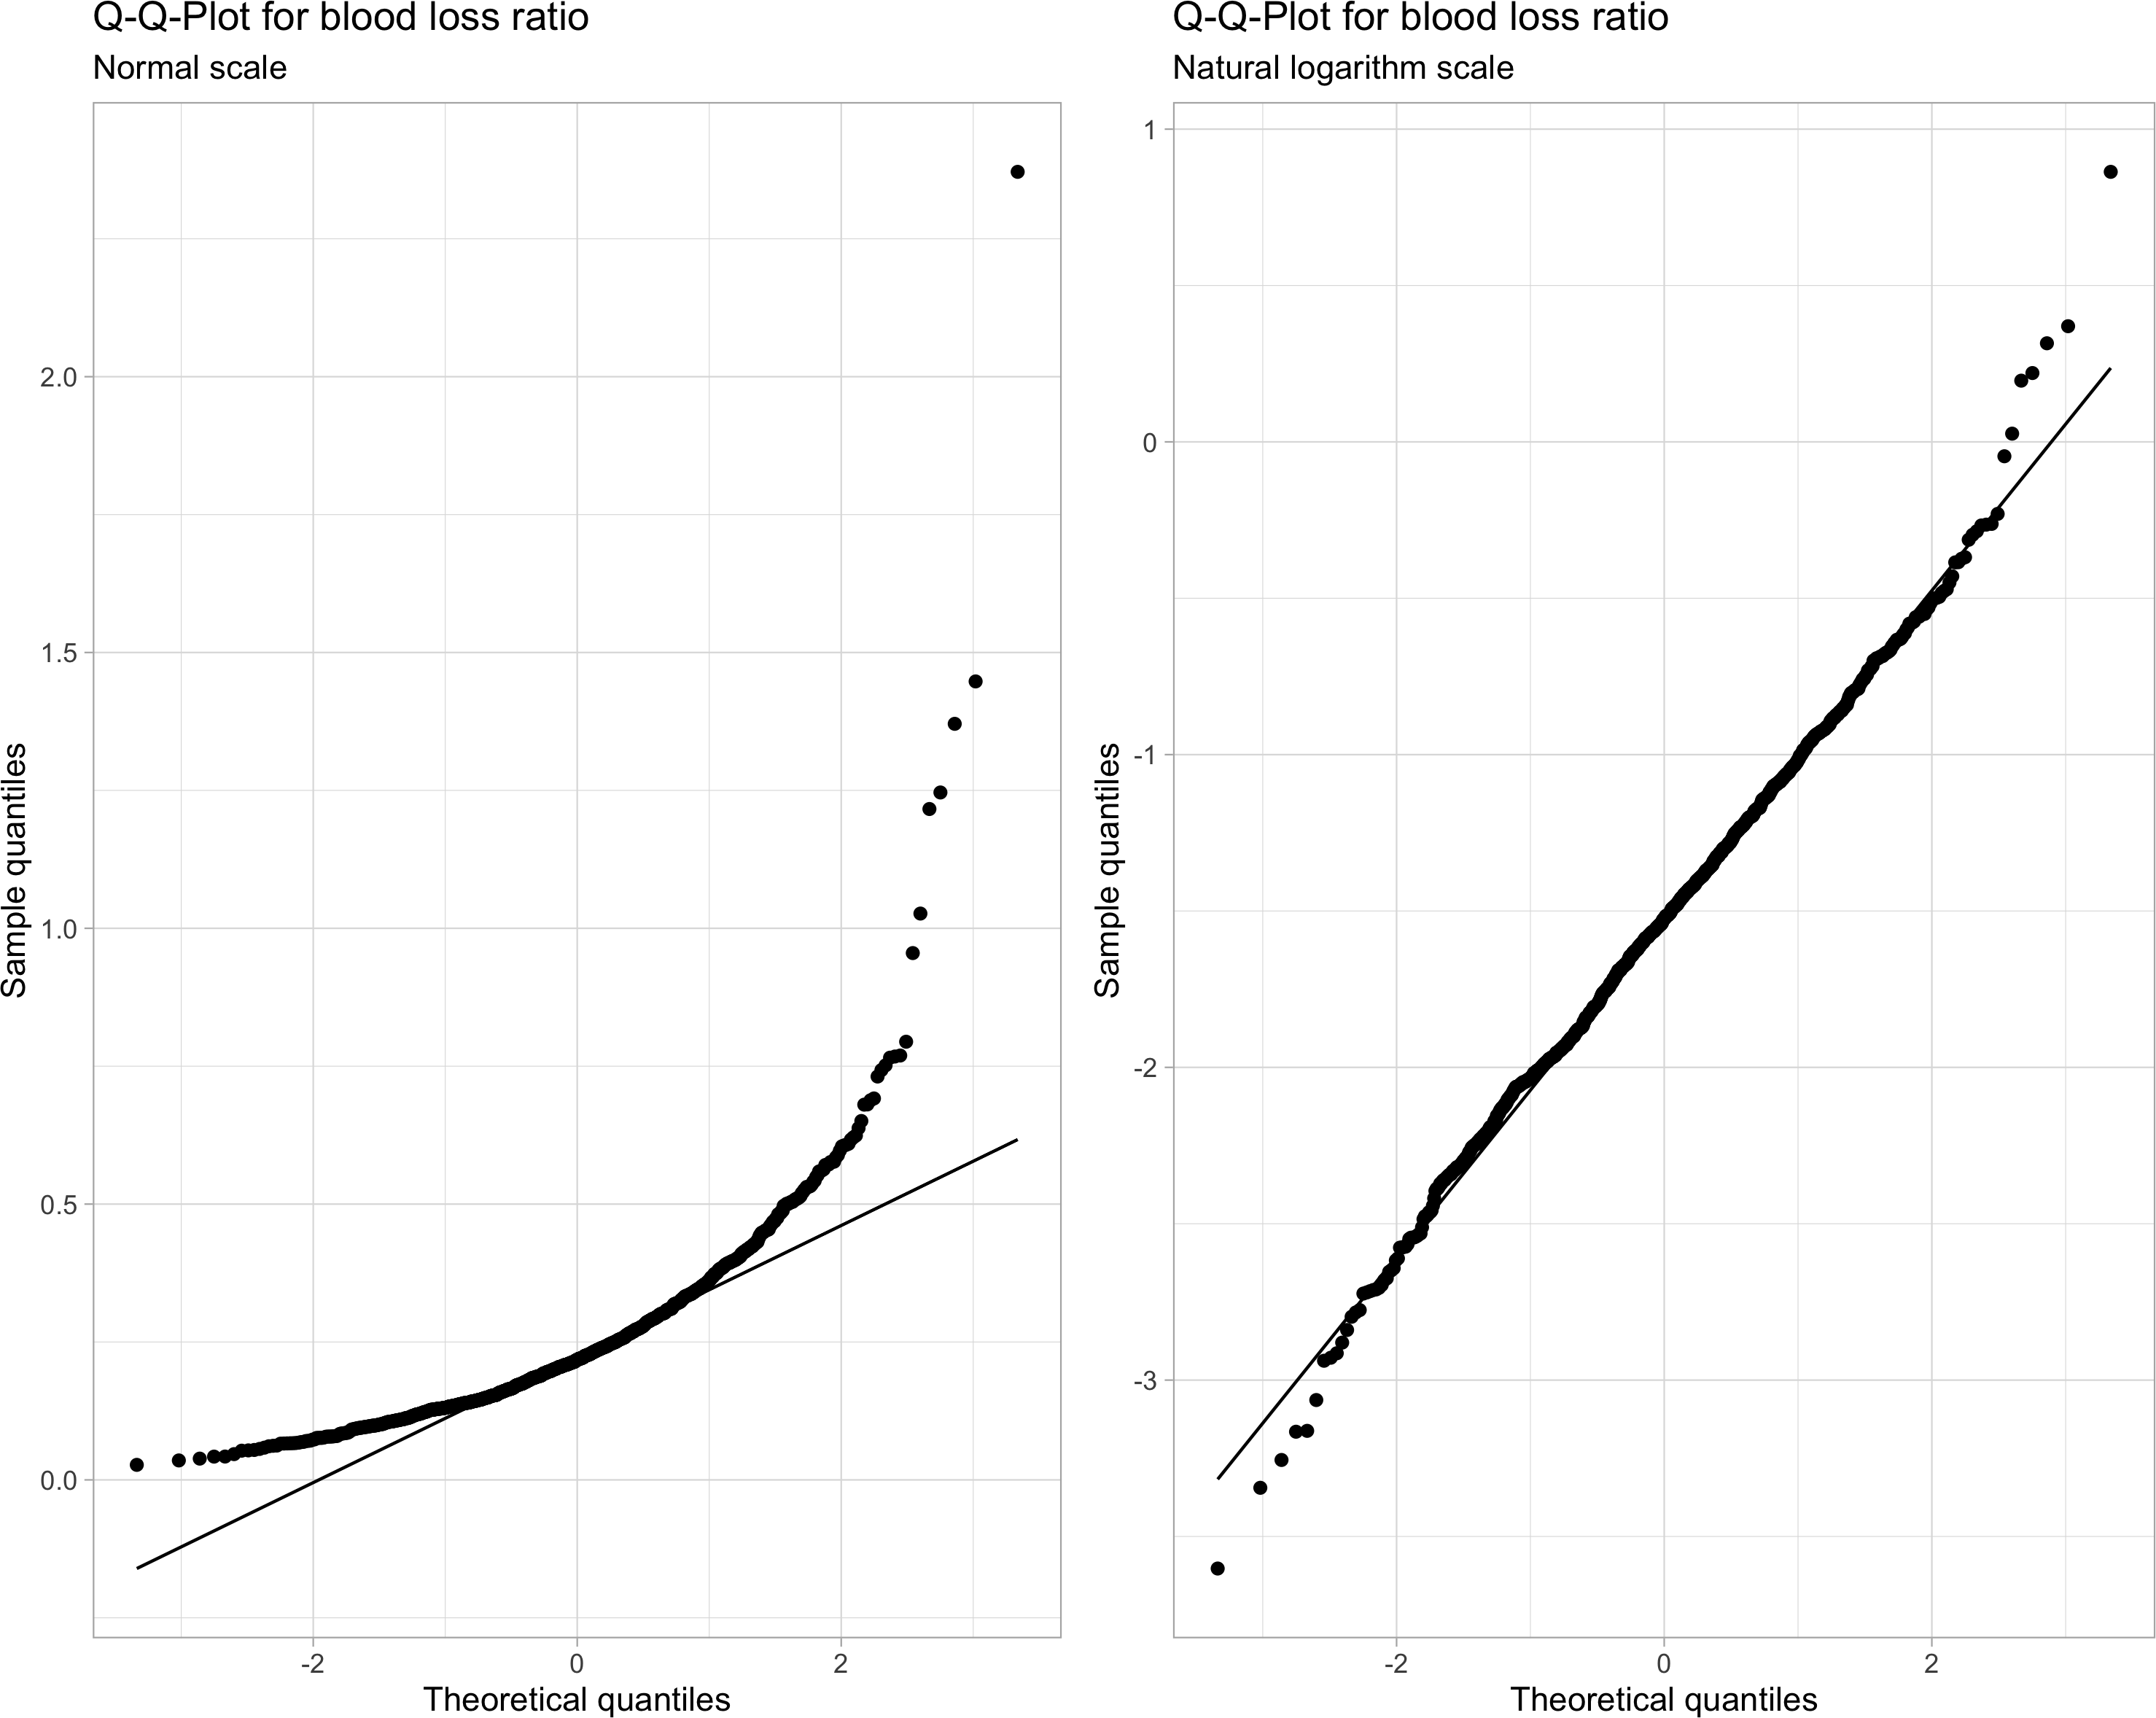
\includegraphics[width=1\linewidth]{notebook_files/figure-latex/data_plots-1} \end{center}

\begin{center}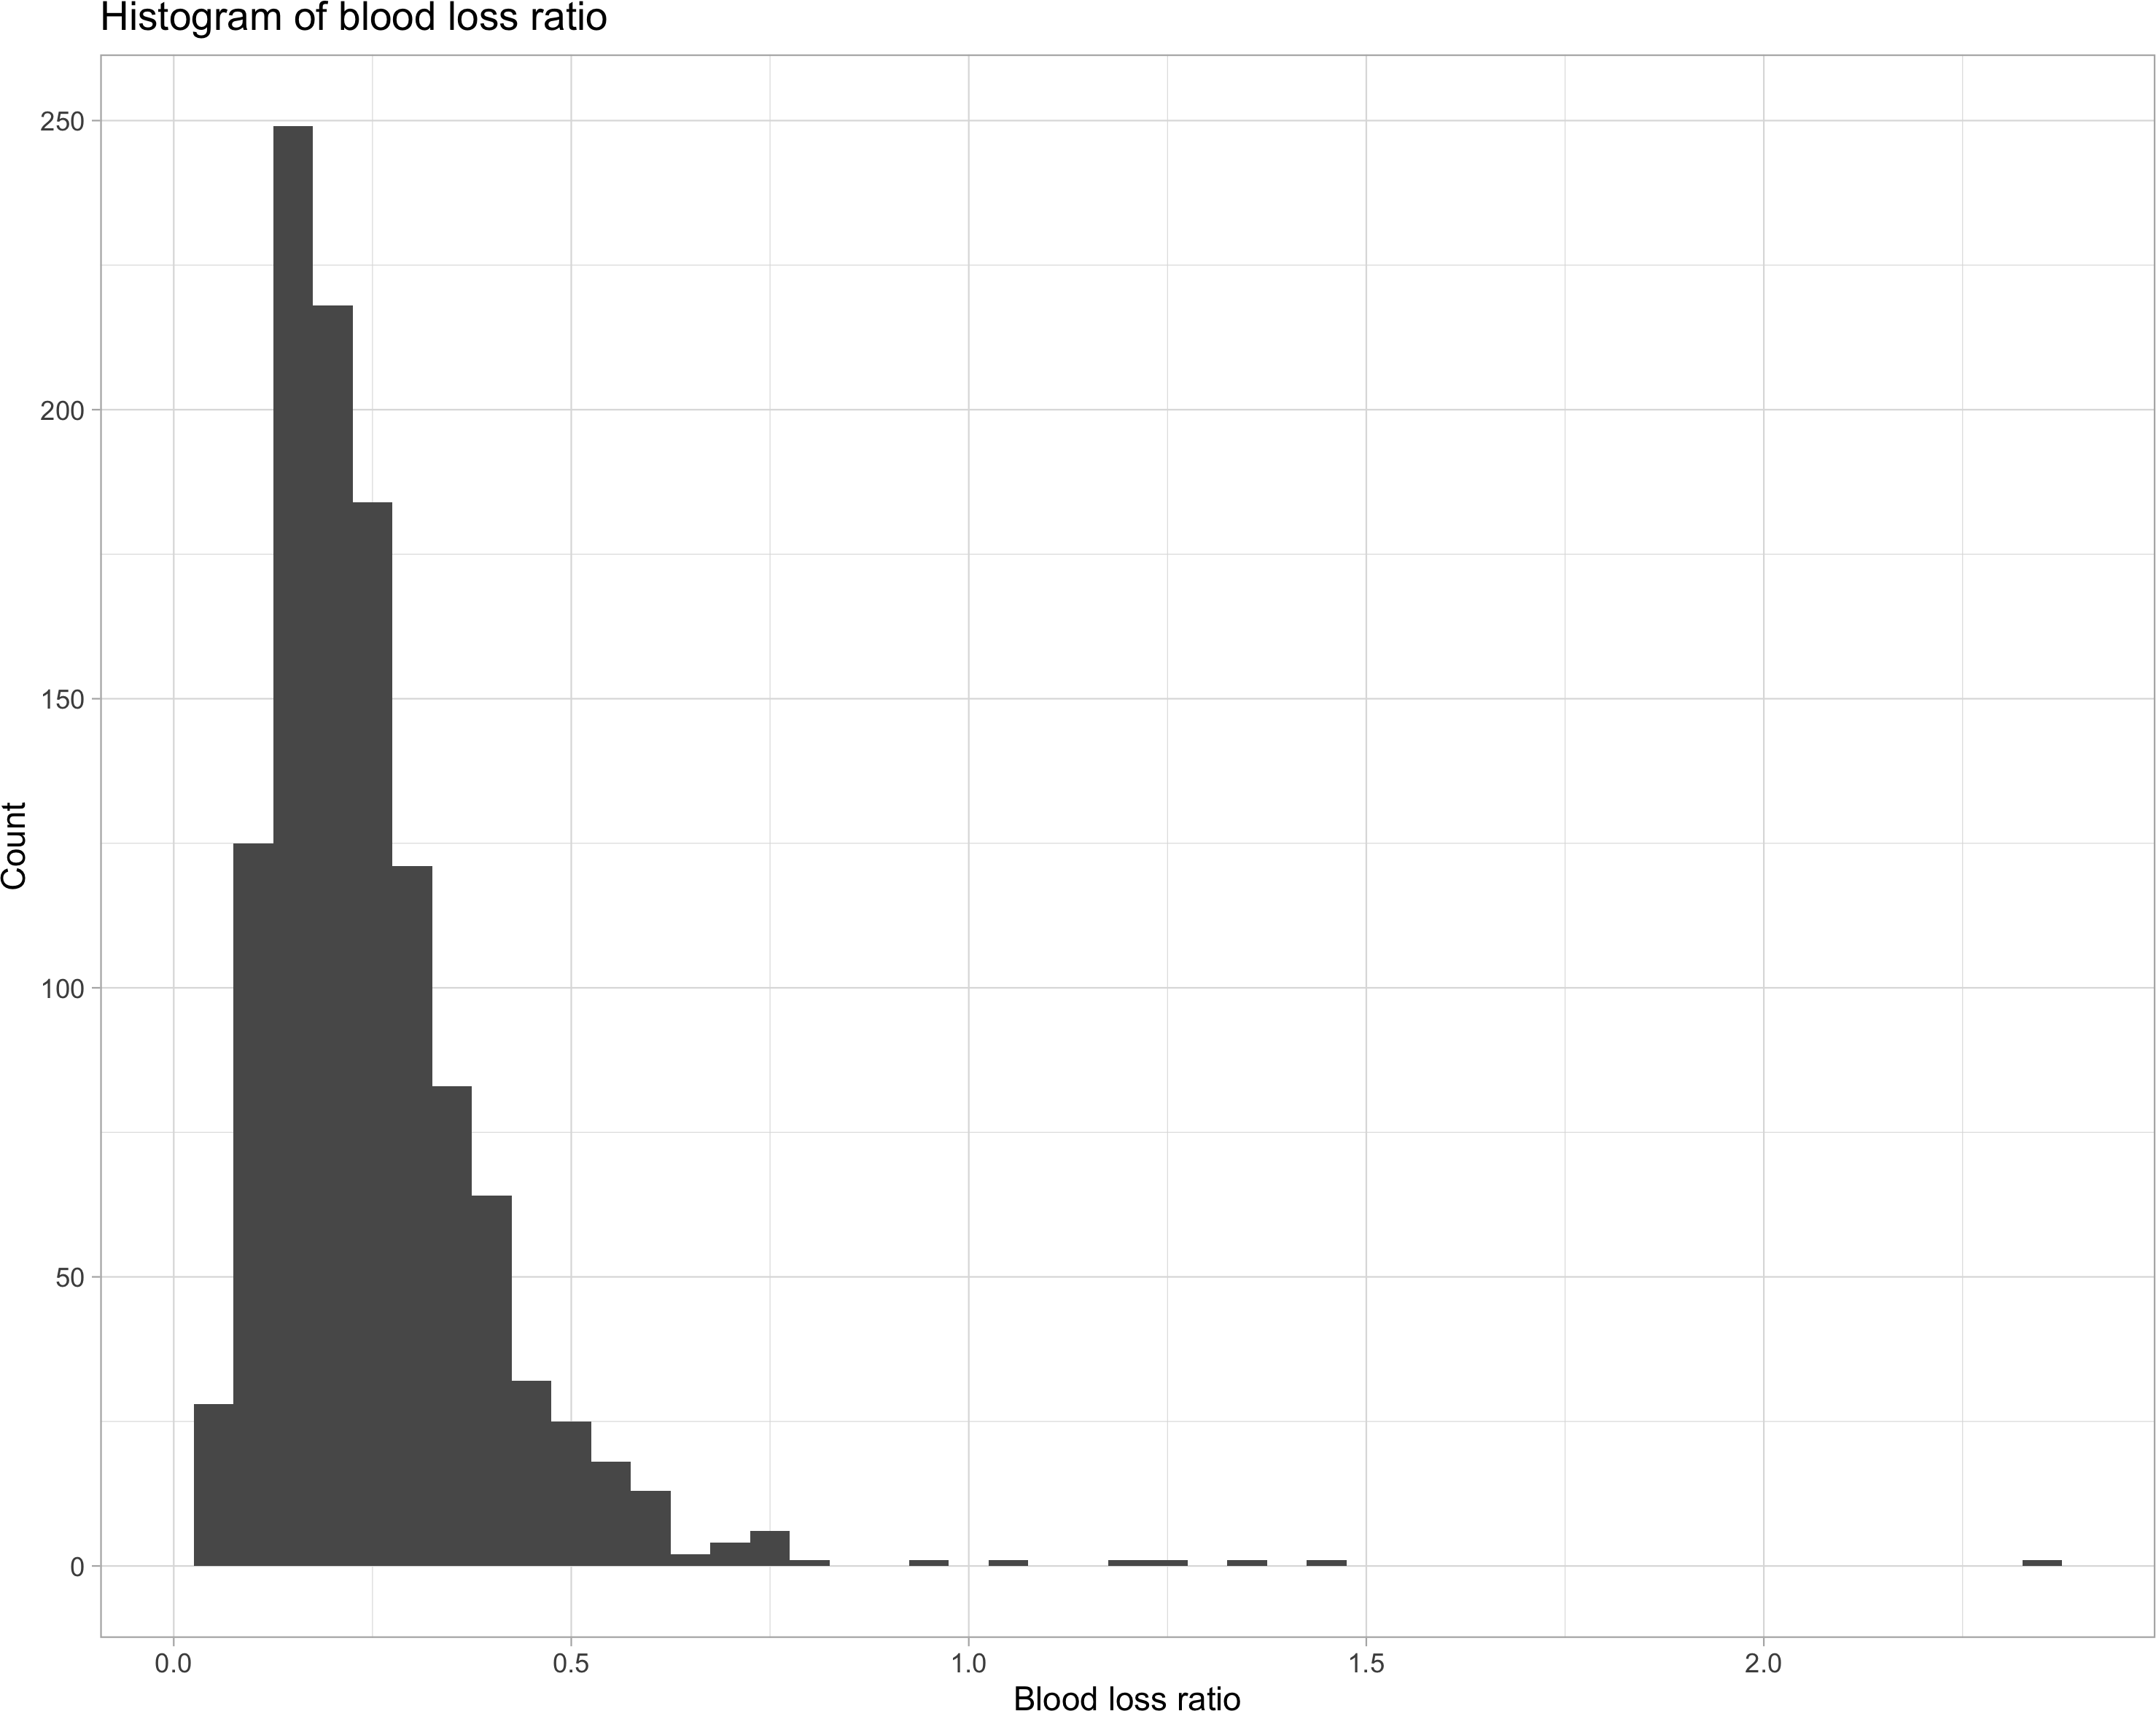
\includegraphics[width=1\linewidth]{notebook_files/figure-latex/data_plots-2} \end{center}

\begin{center}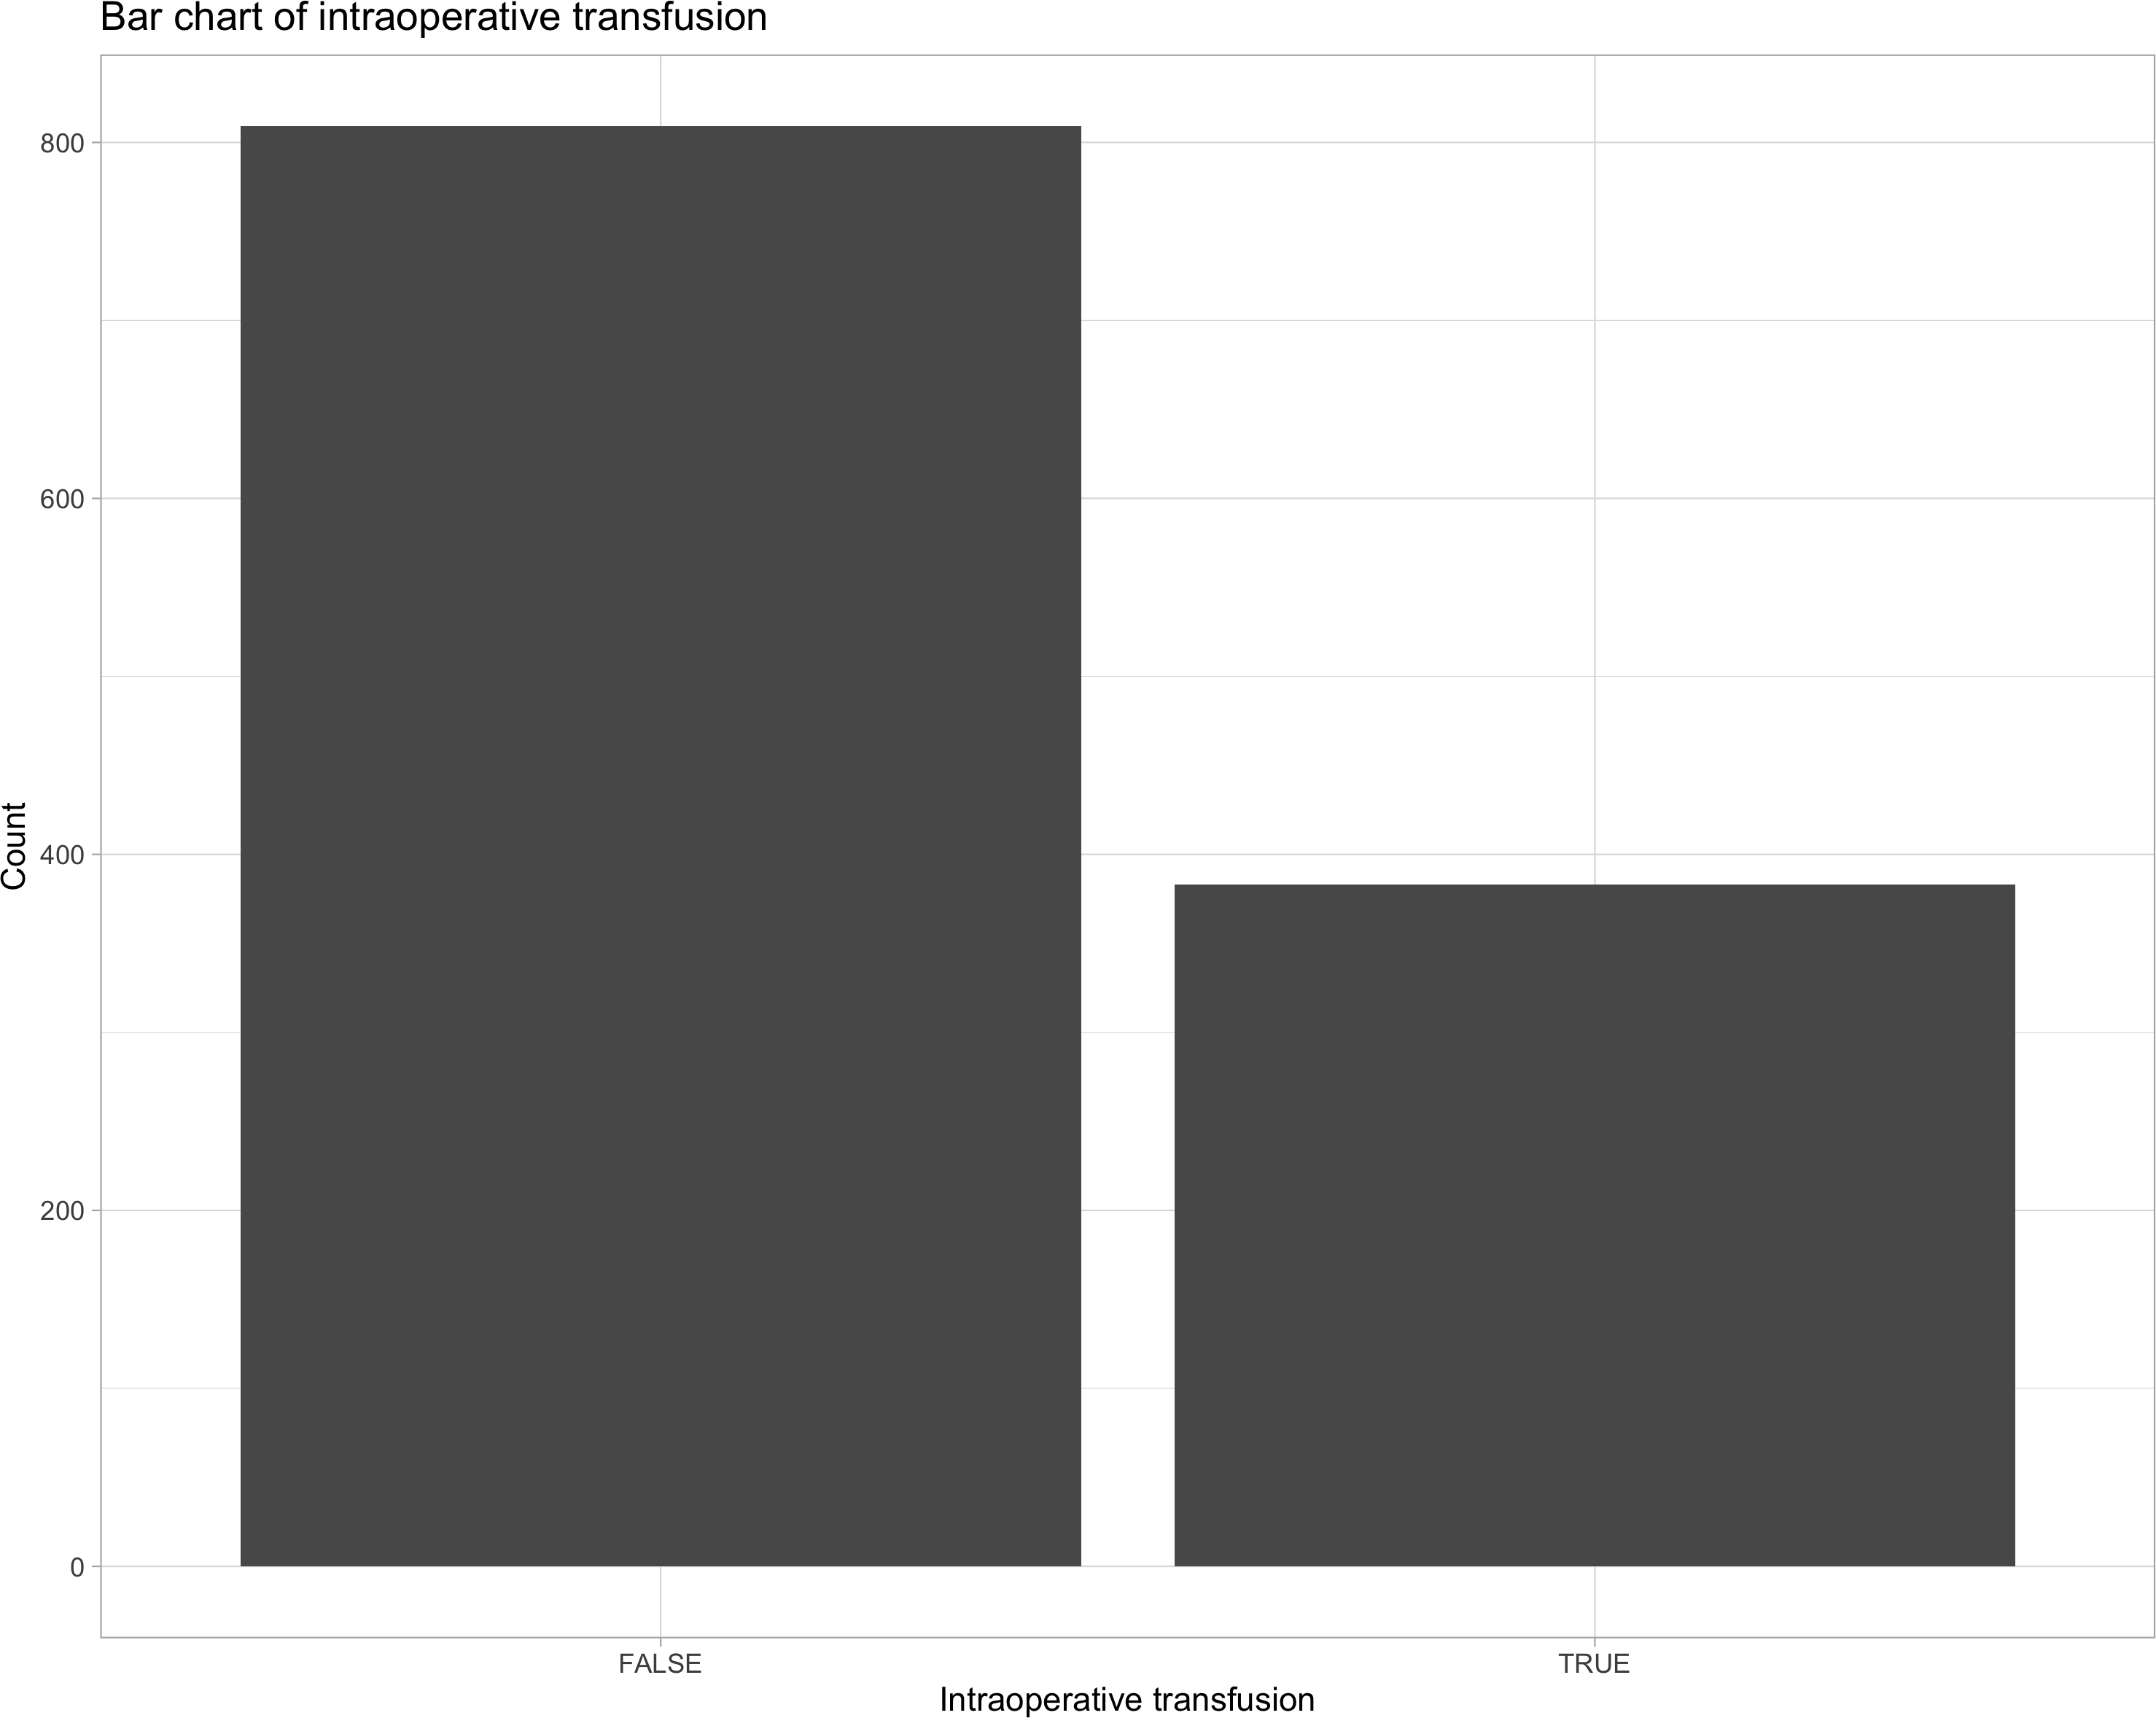
\includegraphics[width=1\linewidth]{notebook_files/figure-latex/data_plots-3} \end{center}

\hypertarget{model-outputs}{%
\subsection{Model outputs}\label{model-outputs}}

\hypertarget{models-with-intraoperative-transfusion-as-response}{%
\subsubsection{Models with intraoperative transfusion as response}\label{models-with-intraoperative-transfusion-as-response}}

\hypertarget{full-model}{%
\paragraph{Full model}\label{full-model}}

\hypertarget{diagnostics}{%
\subparagraph{Diagnostics}\label{diagnostics}}

\begin{verbatim}
#> No divergences to plot.
\end{verbatim}

\begin{center}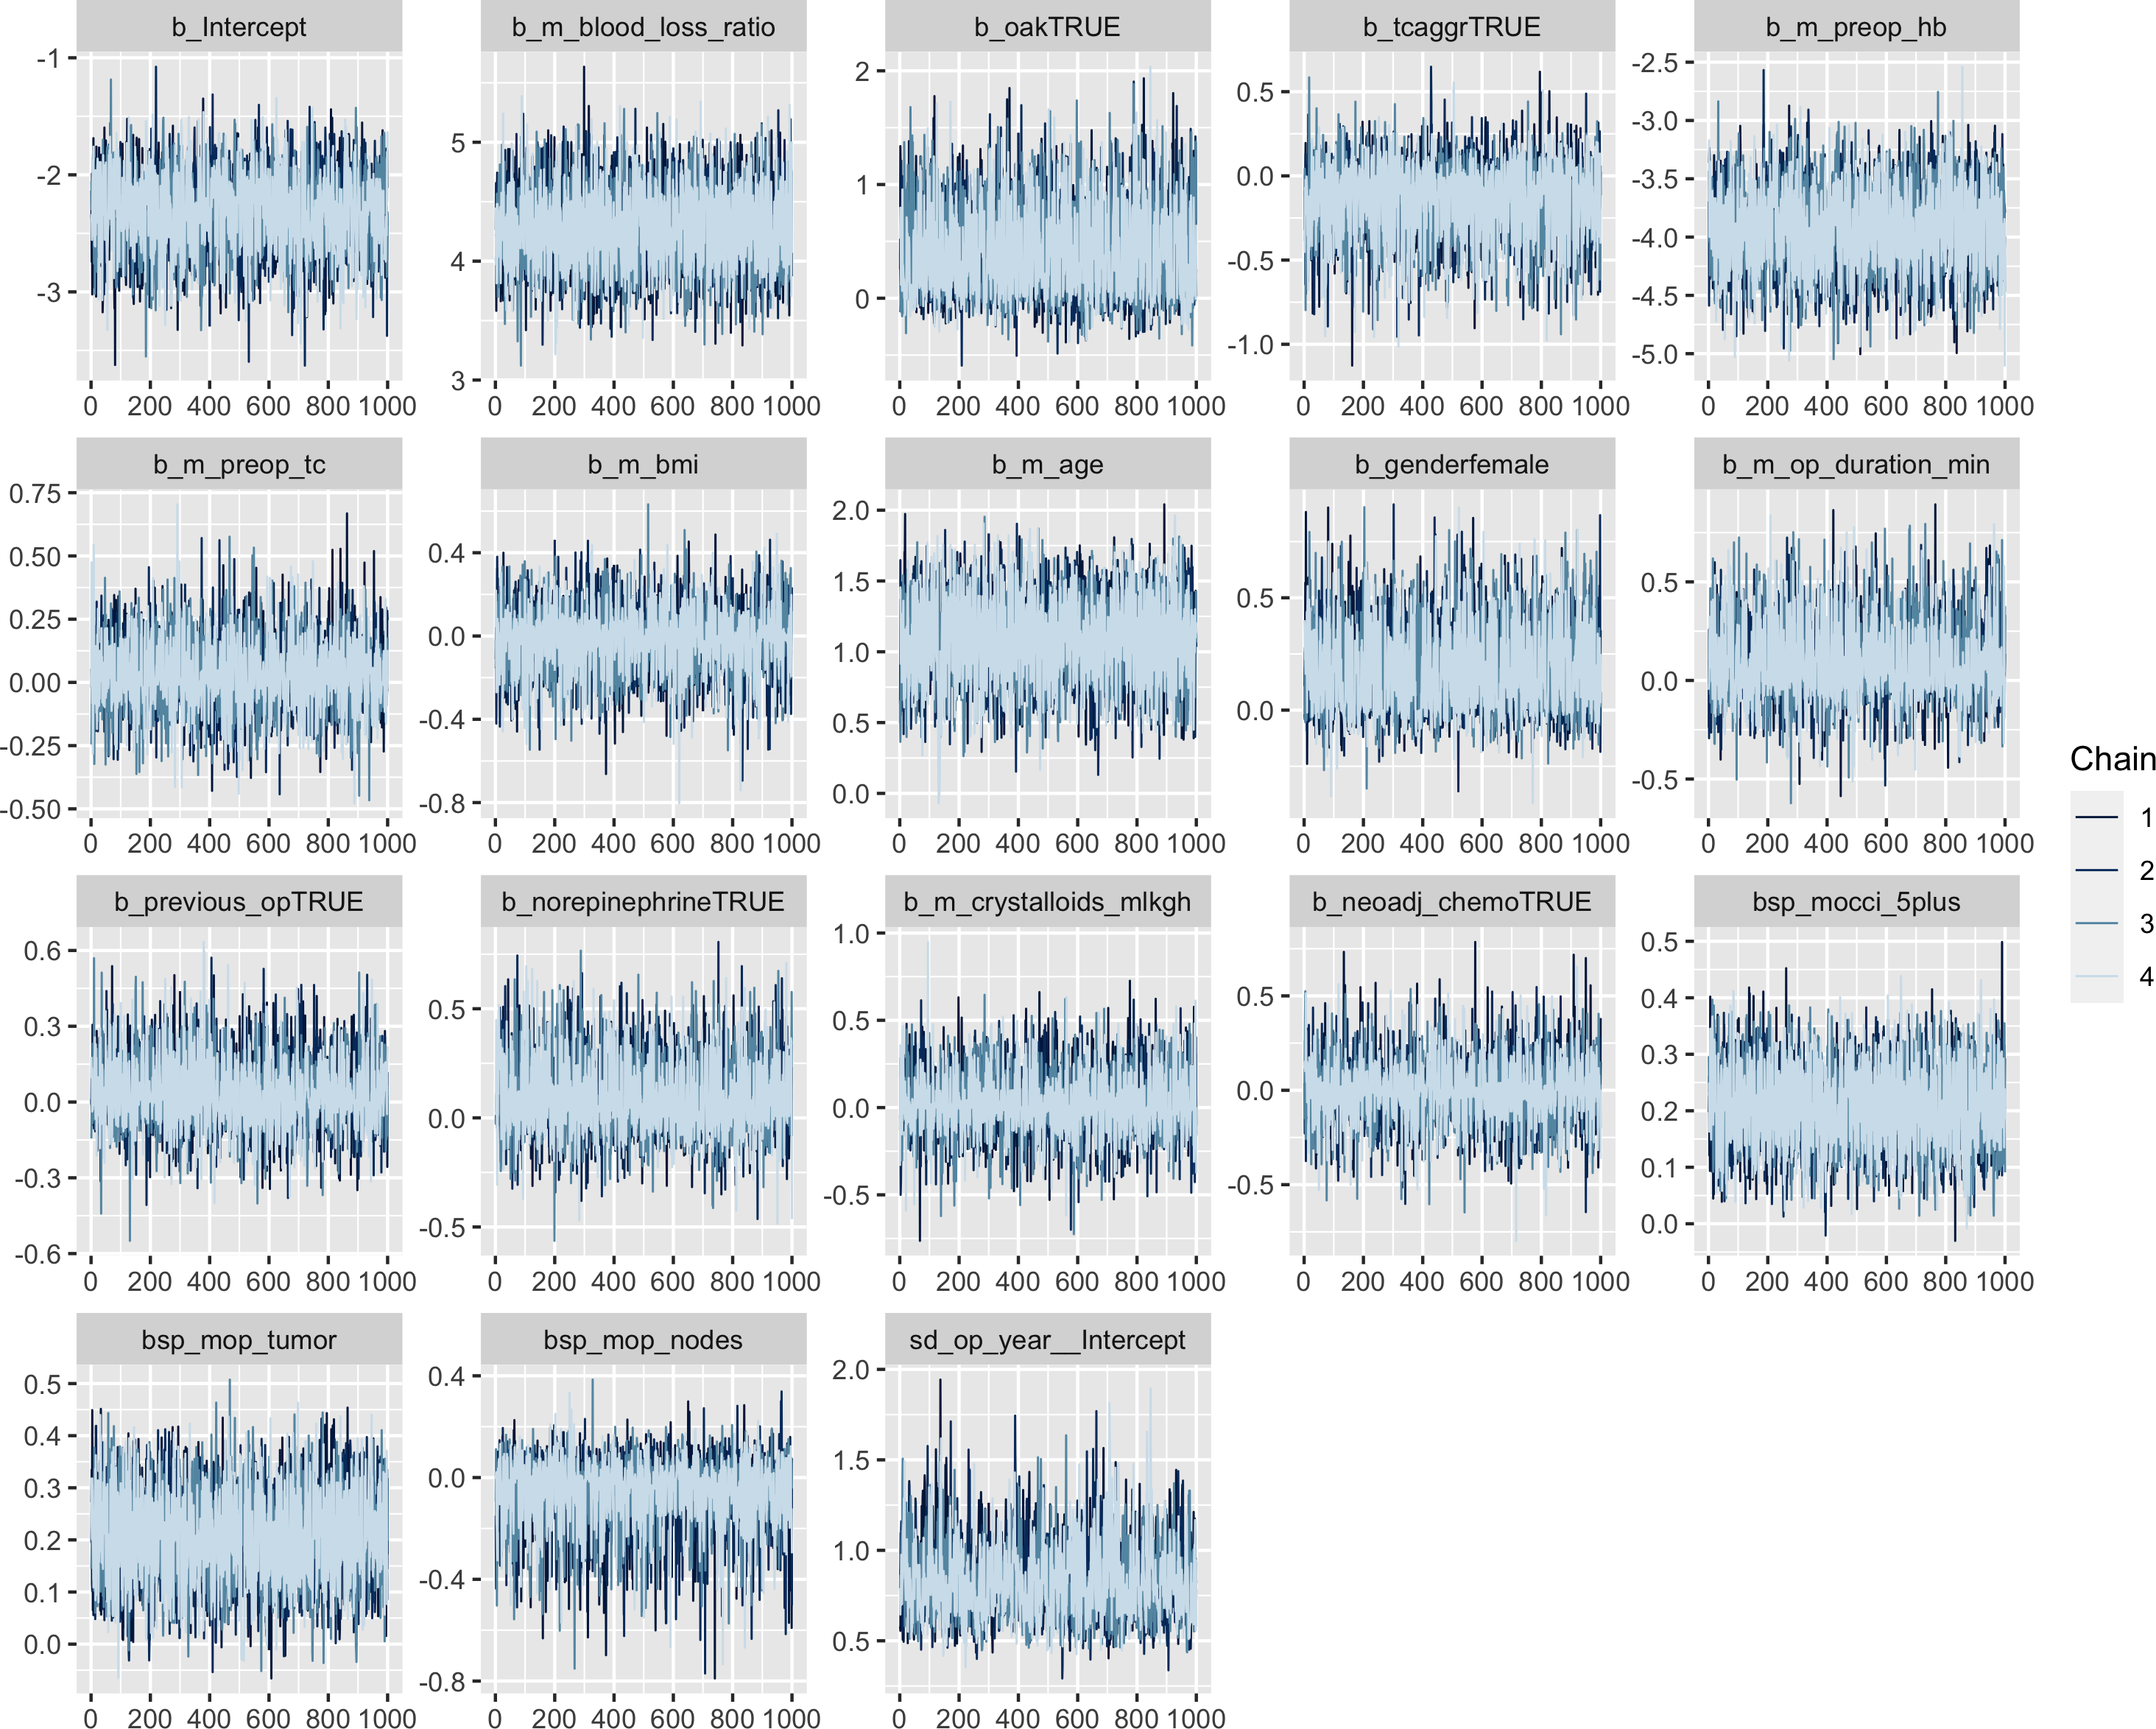
\includegraphics[width=1\linewidth]{notebook_files/figure-latex/model1full_diagnostics-1} \end{center}

\begin{center}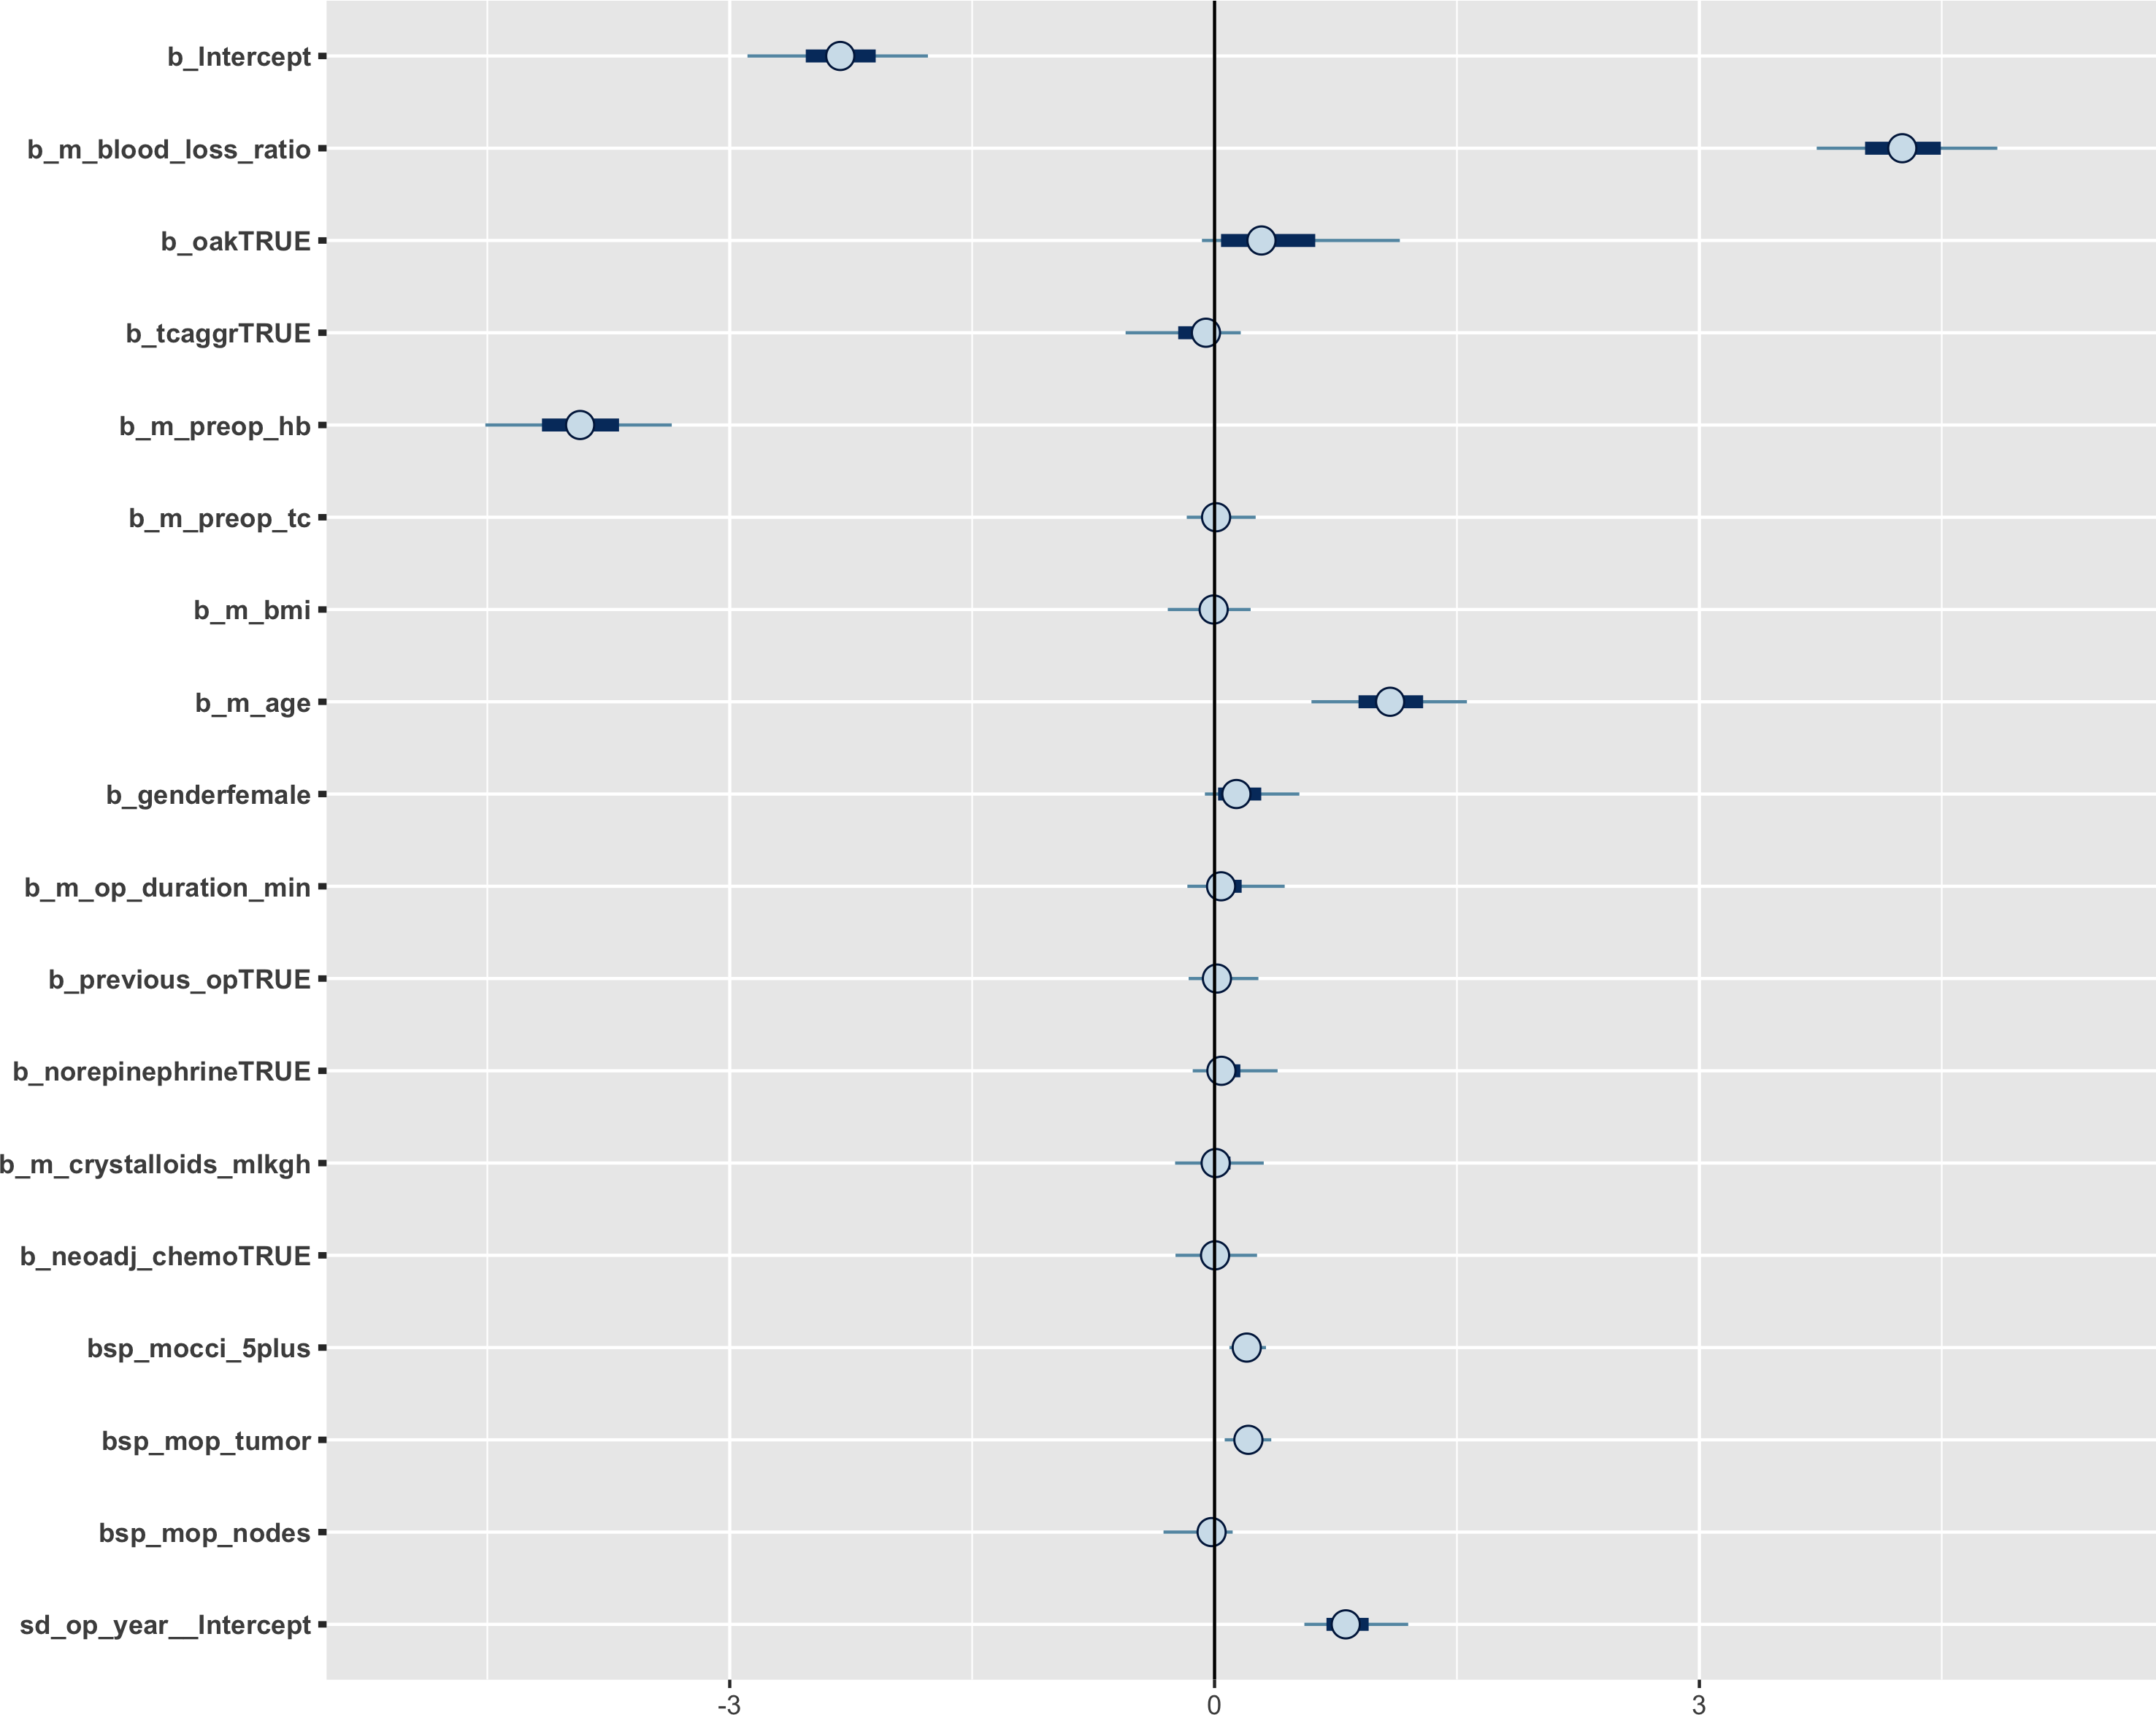
\includegraphics[width=1\linewidth]{notebook_files/figure-latex/model1full_diagnostics-2} \end{center}

\hypertarget{posterior-predictive-check-plot}{%
\subparagraph{Posterior predictive check plot}\label{posterior-predictive-check-plot}}

\begin{verbatim}
#> Using 10 posterior samples for ppc type 'bars' by default.
\end{verbatim}

\begin{center}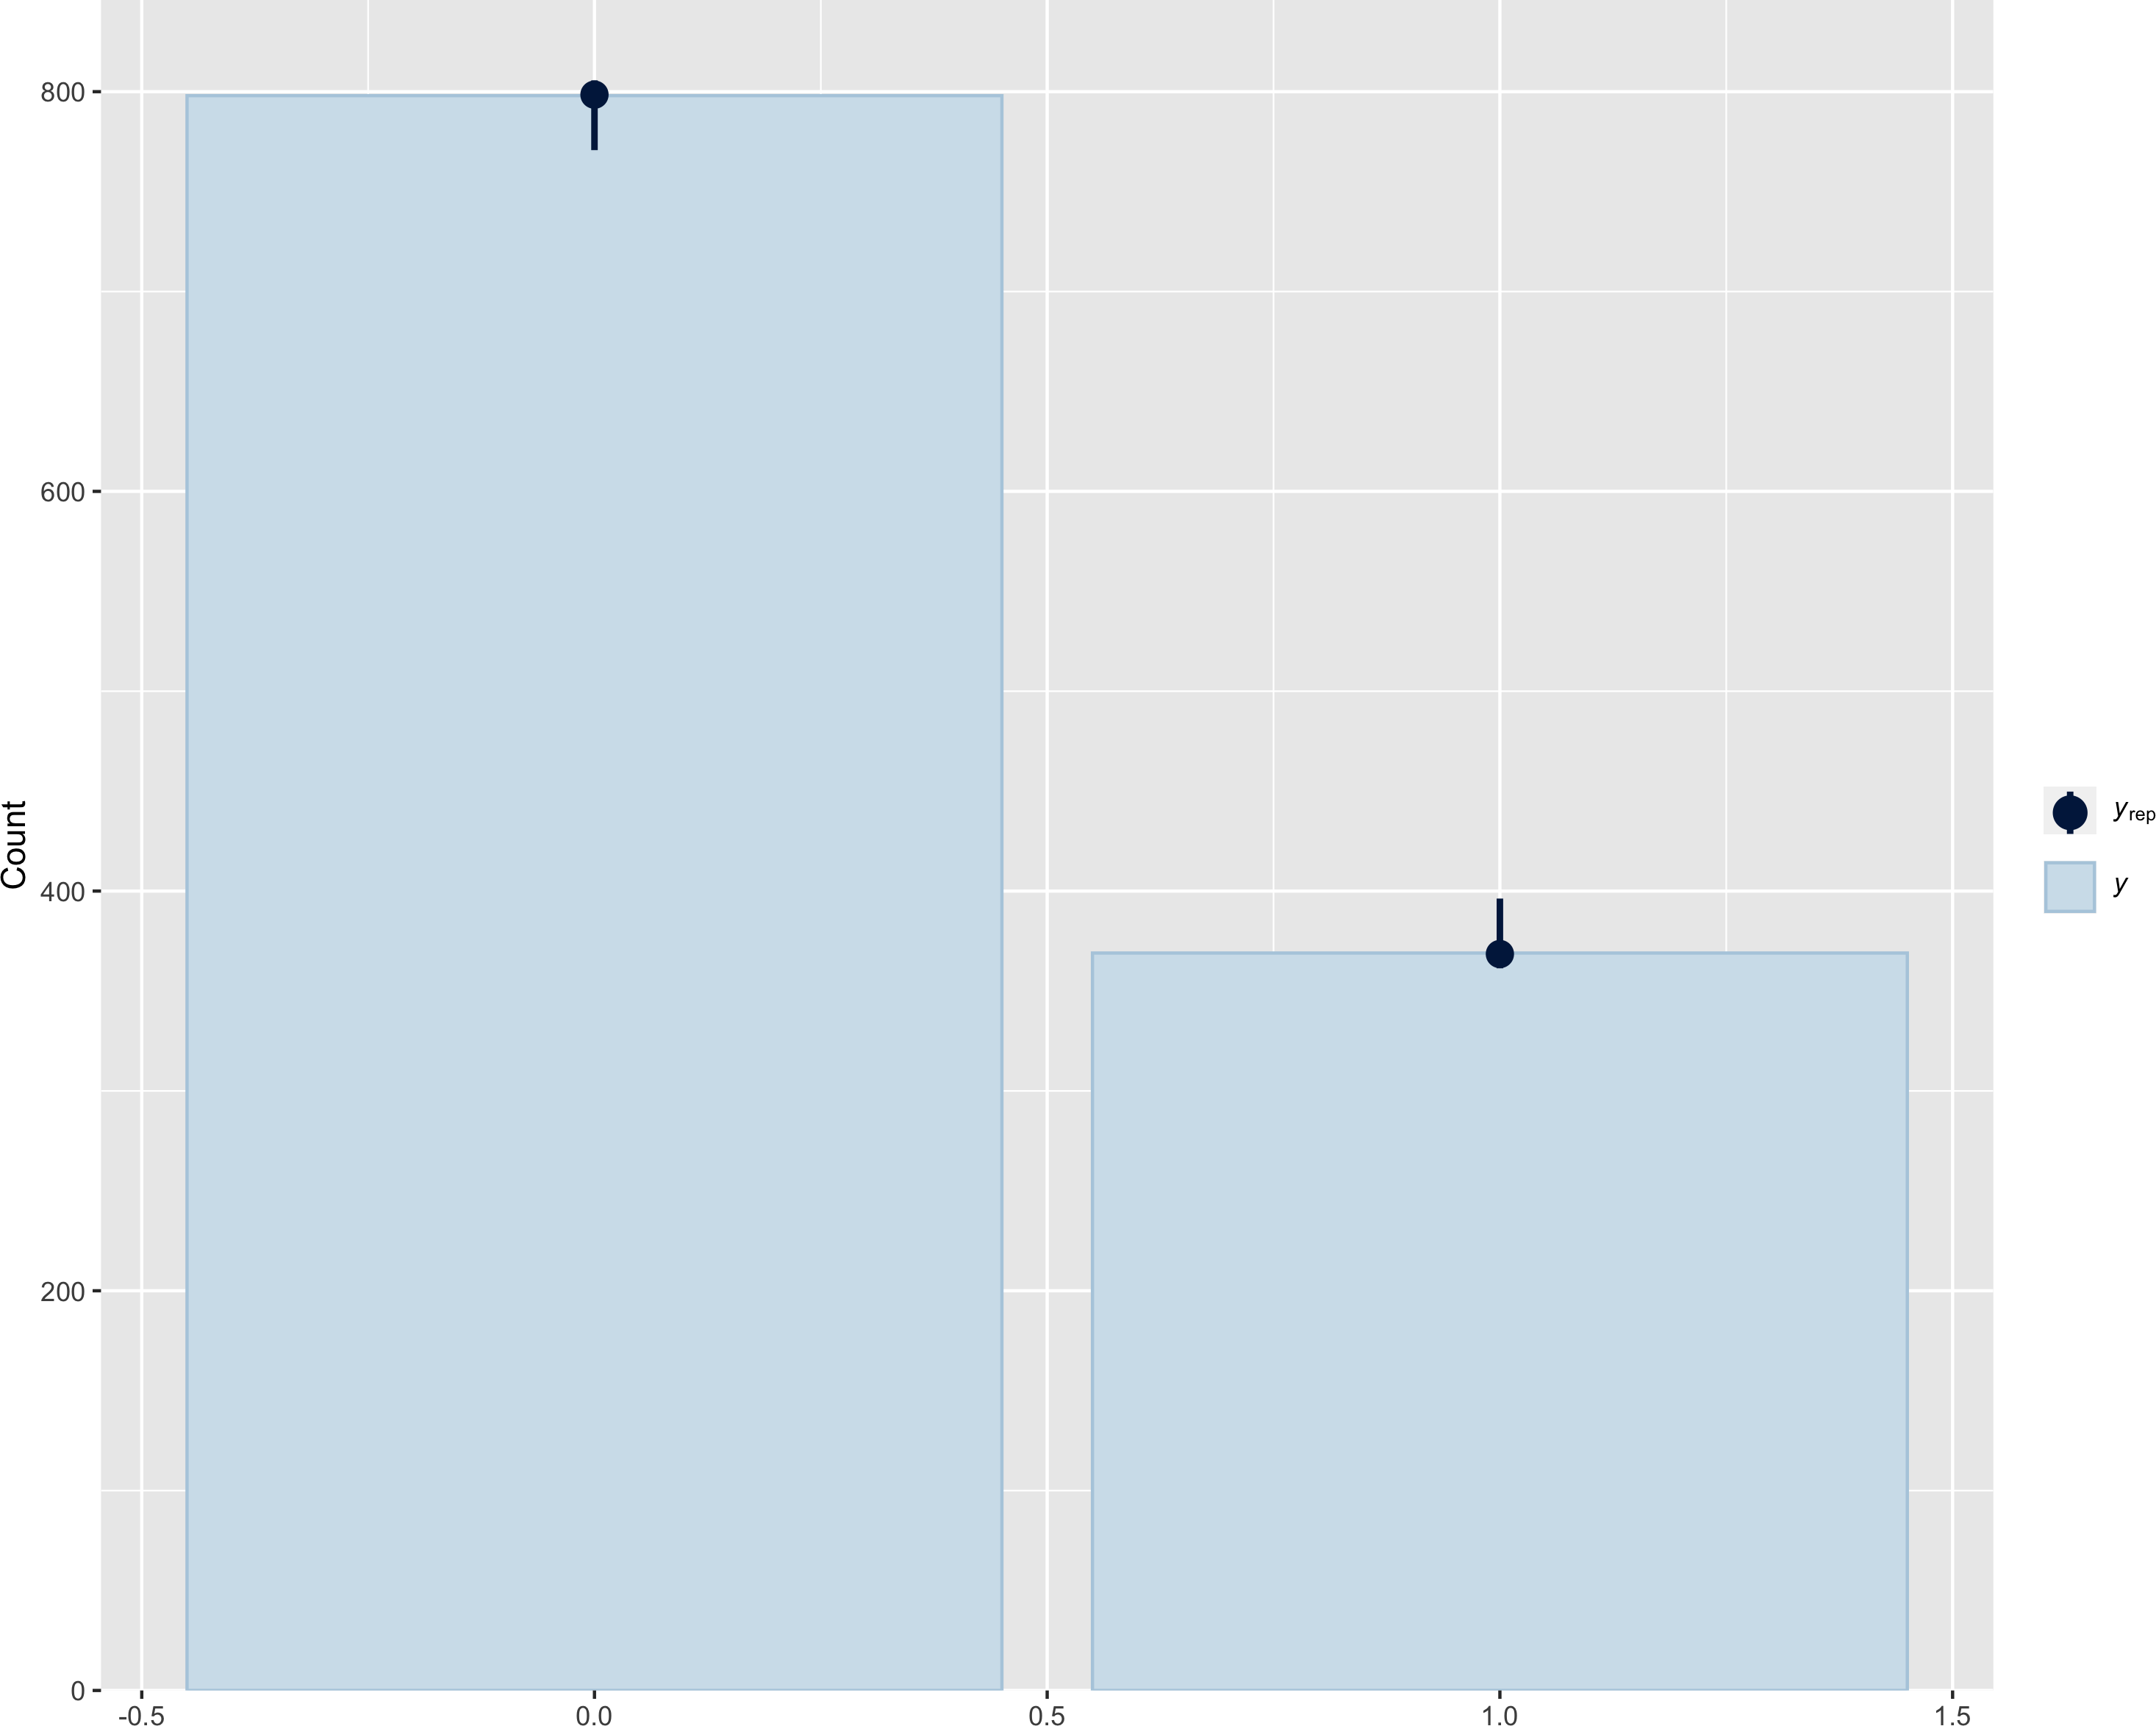
\includegraphics[width=1\linewidth]{notebook_files/figure-latex/model1full_ppcheck-1} \end{center}

\hypertarget{summary}{%
\subparagraph{Summary}\label{summary}}

\begin{verbatim}
#> # Description of Posterior Distributions
#> 
#> Parameter            | Median |           95% CI | p_MAP |    pd |       100% ROPE | % in ROPE
#> ----------------------------------------------------------------------------------------------
#> Intercept            | -2.316 | [-2.976, -1.652] | 0.000 | 1.000 | [-0.055, 0.055] |     0.000
#> m_blood_loss_ratio   |  4.256 | [ 3.619,  4.937] | 0.000 | 1.000 | [-0.055, 0.055] |     0.000
#> oakTRUE              |  0.290 | [-0.207,  1.212] | 0.987 | 0.845 | [-0.055, 0.055] |    20.600
#> tcaggrTRUE           | -0.053 | [-0.605,  0.275] | 0.997 | 0.691 | [-0.055, 0.055] |    35.425
#> m_preop_hb           | -3.926 | [-4.657, -3.283] | 0.000 | 1.000 | [-0.055, 0.055] |     0.000
#> m_preop_tc           |  0.009 | [-0.218,  0.304] | 1.000 | 0.567 | [-0.055, 0.055] |    46.200
#> m_bmi                | -0.006 | [-0.360,  0.274] | 0.997 | 0.539 | [-0.055, 0.055] |    42.175
#> m_age                |  1.086 | [ 0.536,  1.689] | 0.007 | 0.999 | [-0.055, 0.055] |     0.125
#> genderfemale         |  0.135 | [-0.124,  0.574] | 0.988 | 0.824 | [-0.055, 0.055] |    27.950
#> m_op_duration_min    |  0.040 | [-0.266,  0.486] | 0.999 | 0.655 | [-0.055, 0.055] |    37.625
#> previous_opTRUE      |  0.015 | [-0.223,  0.310] | 0.999 | 0.590 | [-0.055, 0.055] |    46.550
#> norepinephrineTRUE   |  0.042 | [-0.201,  0.433] | 0.999 | 0.674 | [-0.055, 0.055] |    38.925
#> m_crystalloids_mlkgh |  0.007 | [-0.325,  0.370] | 1.000 | 0.546 | [-0.055, 0.055] |    40.975
#> neoadj_chemoTRUE     |  0.003 | [-0.326,  0.322] | 0.996 | 0.525 | [-0.055, 0.055] |    43.350
#> mocci_5plus          |  0.199 | [ 0.068,  0.338] | 0.000 | 1.000 | [-0.055, 0.055] |     1.550
#> mop_tumor            |  0.209 | [ 0.032,  0.374] | 0.085 | 0.991 | [-0.055, 0.055] |     4.225
#> mop_nodes            | -0.018 | [-0.361,  0.166] | 1.000 | 0.616 | [-0.055, 0.055] |    51.125
\end{verbatim}

\hypertarget{region-of-practical-equivalence}{%
\subparagraph{Region of practical equivalence}\label{region-of-practical-equivalence}}

Using a ROPE range of -0.055 to 0.055 (\(0.1 \cdot \frac{\sqrt{3}}{\pi}\)) and a CI of 1.

\begin{center}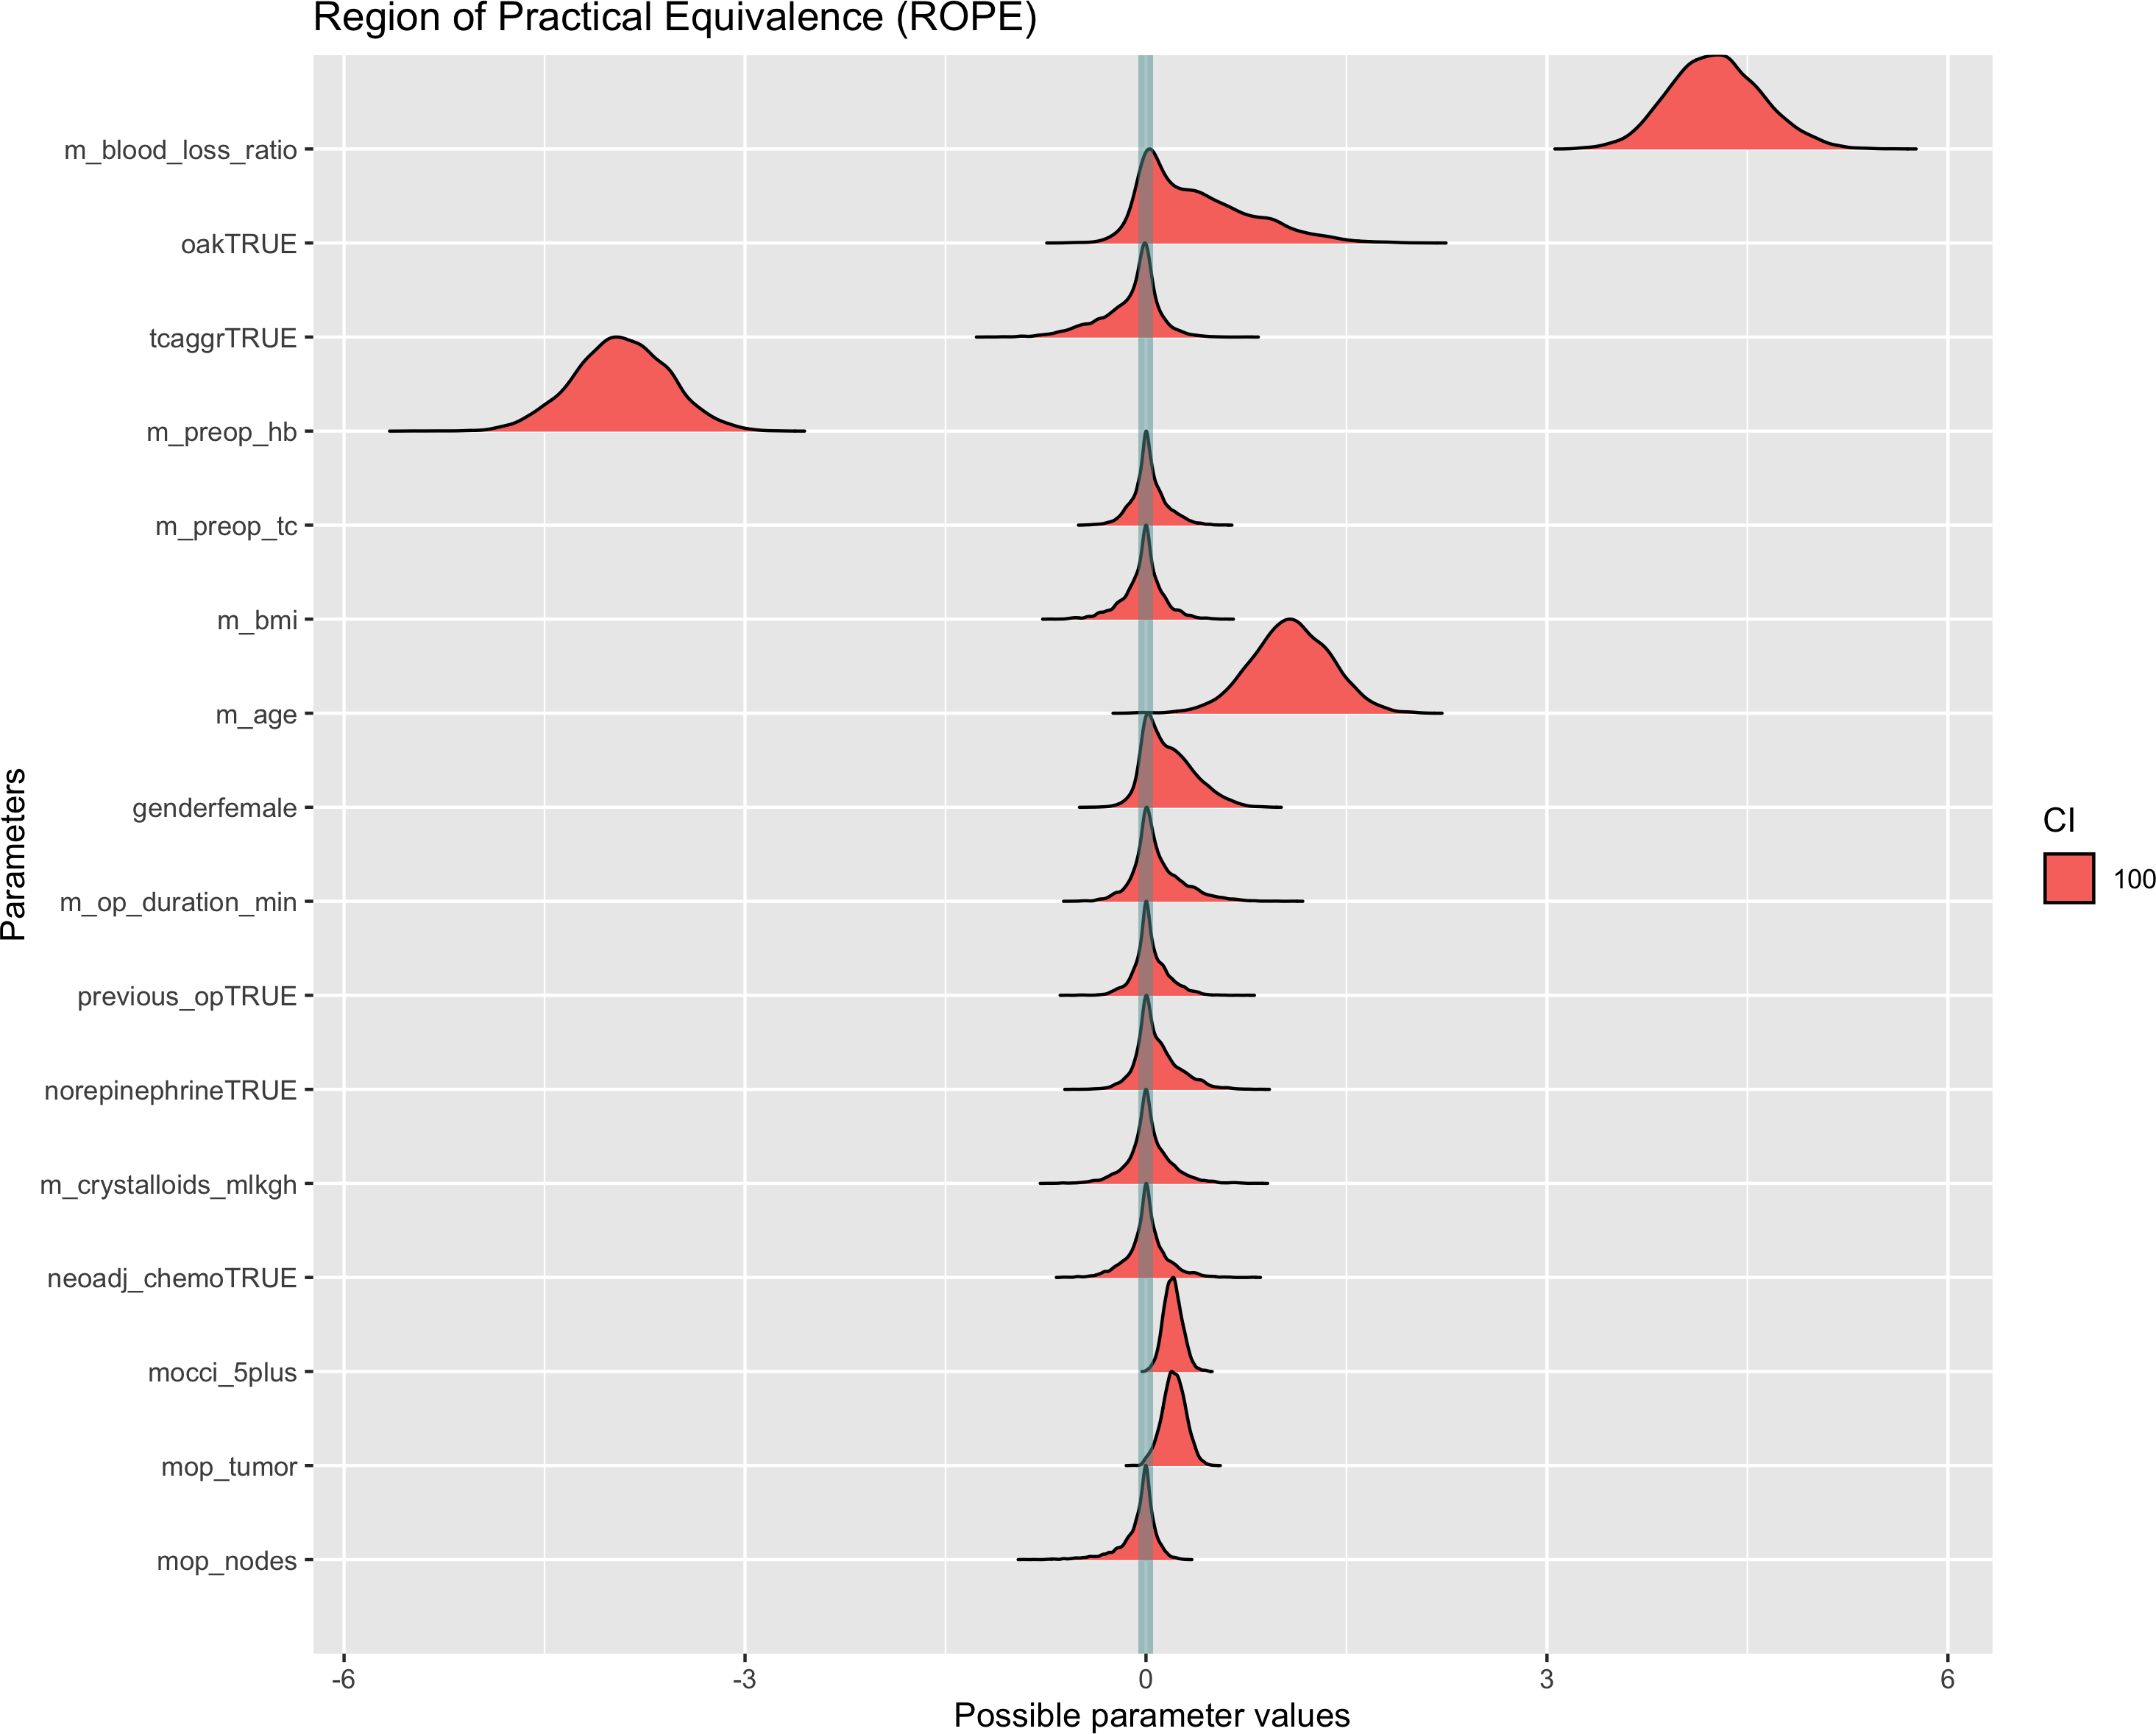
\includegraphics[width=1\linewidth]{notebook_files/figure-latex/model1full_rope-1} \end{center}

\hypertarget{roc-auc}{%
\subparagraph{ROC-AUC}\label{roc-auc}}

\begin{verbatim}
#> AUC: 0.879159280314611
\end{verbatim}

\begin{center}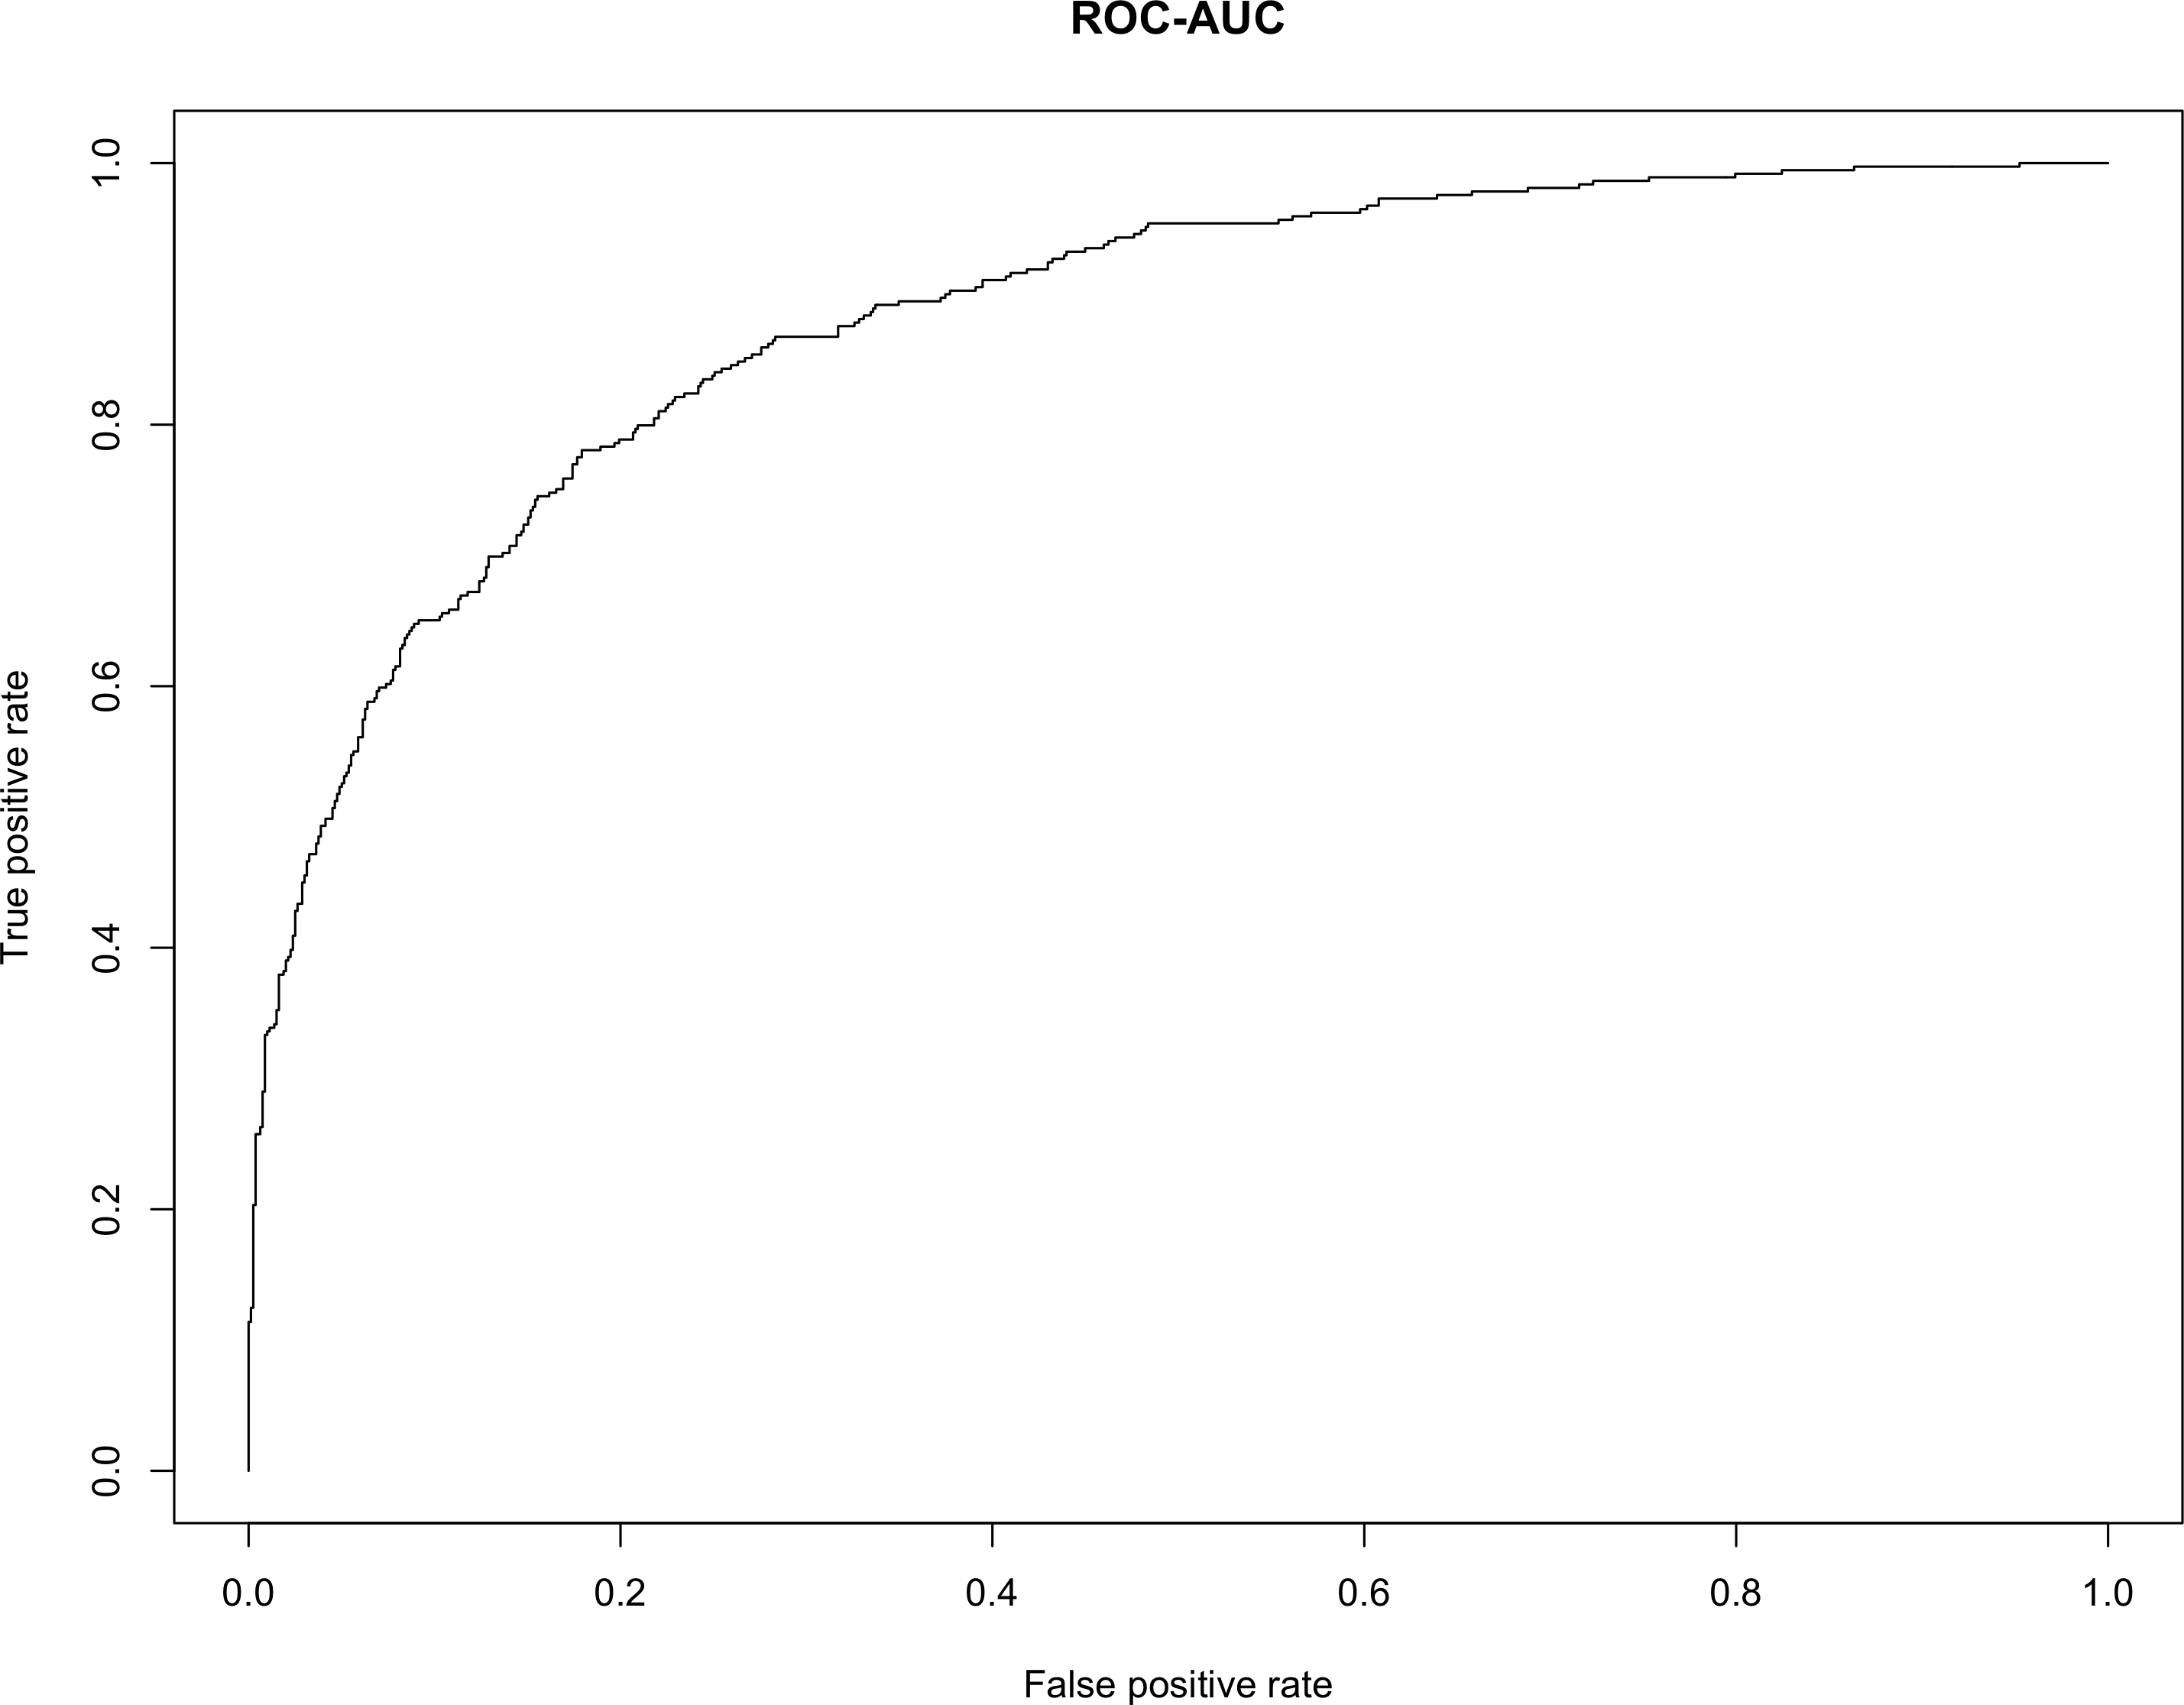
\includegraphics[width=1\linewidth]{notebook_files/figure-latex/model1full_rocauc-1} \end{center}

\hypertarget{conditional-probability-plot}{%
\subparagraph{Conditional probability plot}\label{conditional-probability-plot}}

\hypertarget{reduced-model}{%
\paragraph{Reduced model}\label{reduced-model}}

\hypertarget{diagnostics-1}{%
\subparagraph{Diagnostics}\label{diagnostics-1}}

\begin{verbatim}
#> No divergences to plot.
\end{verbatim}

\begin{center}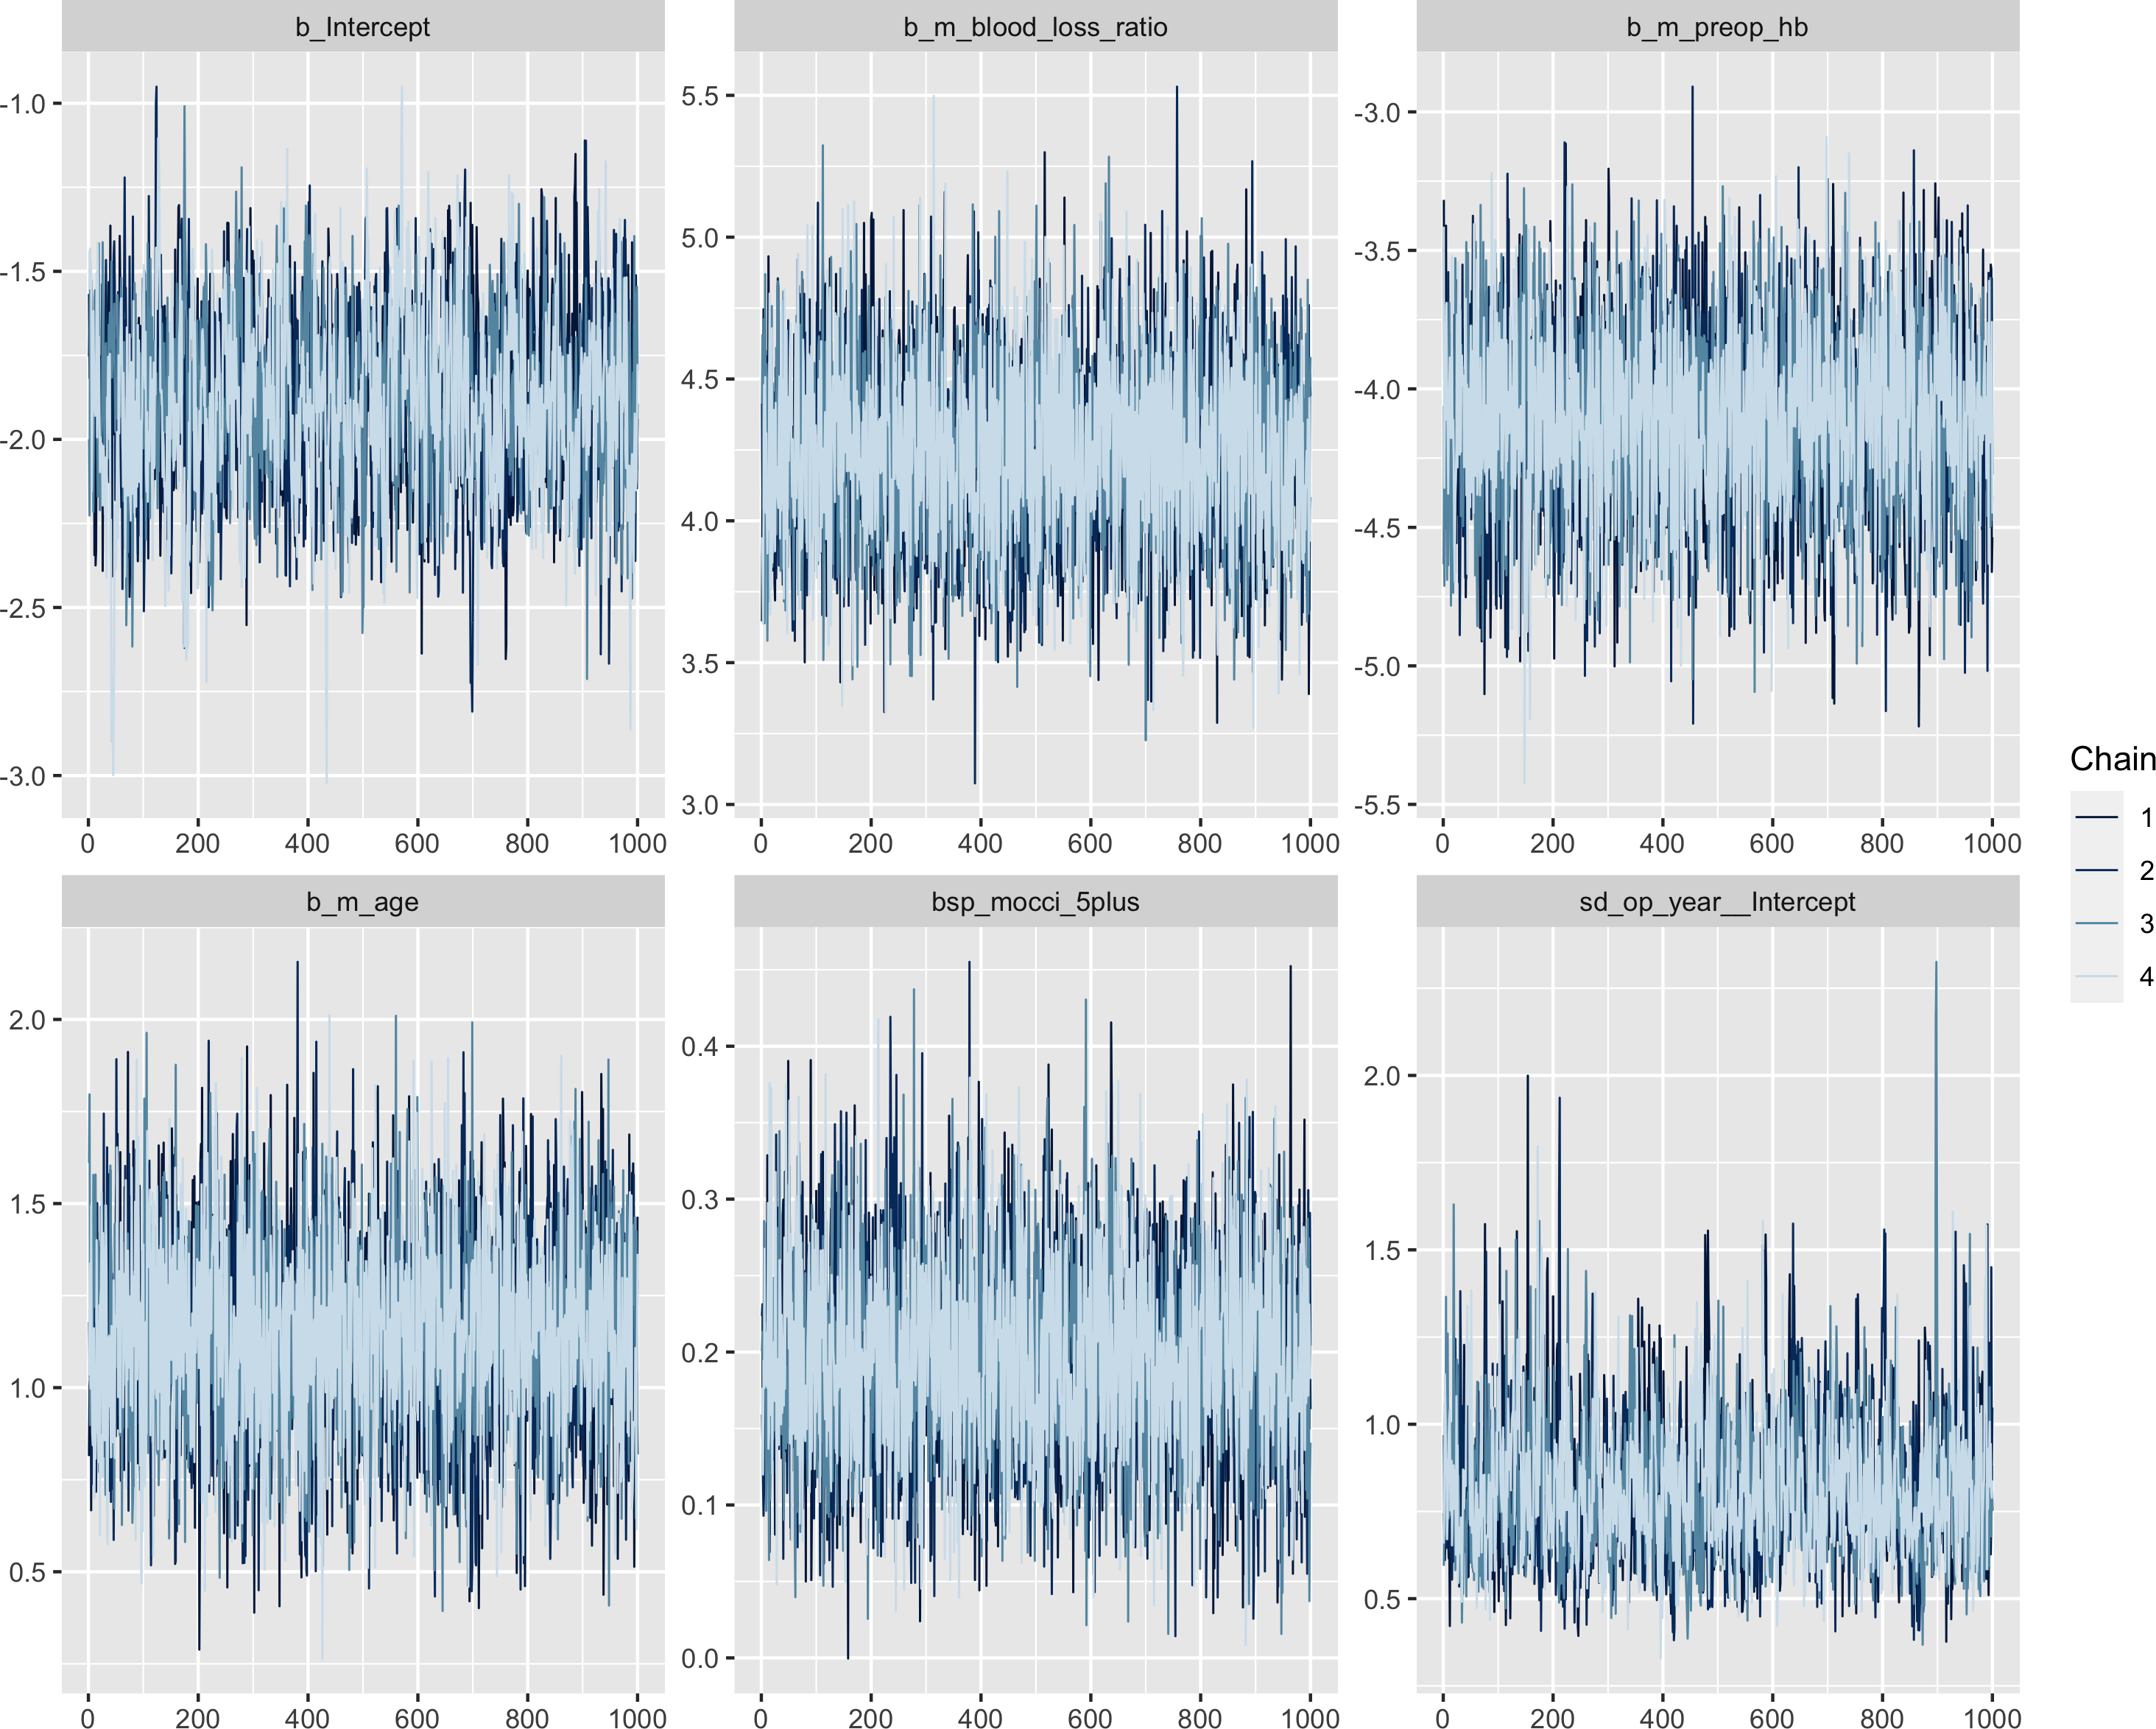
\includegraphics[width=1\linewidth]{notebook_files/figure-latex/model1reduced_diagnostics-1} \end{center}

\begin{center}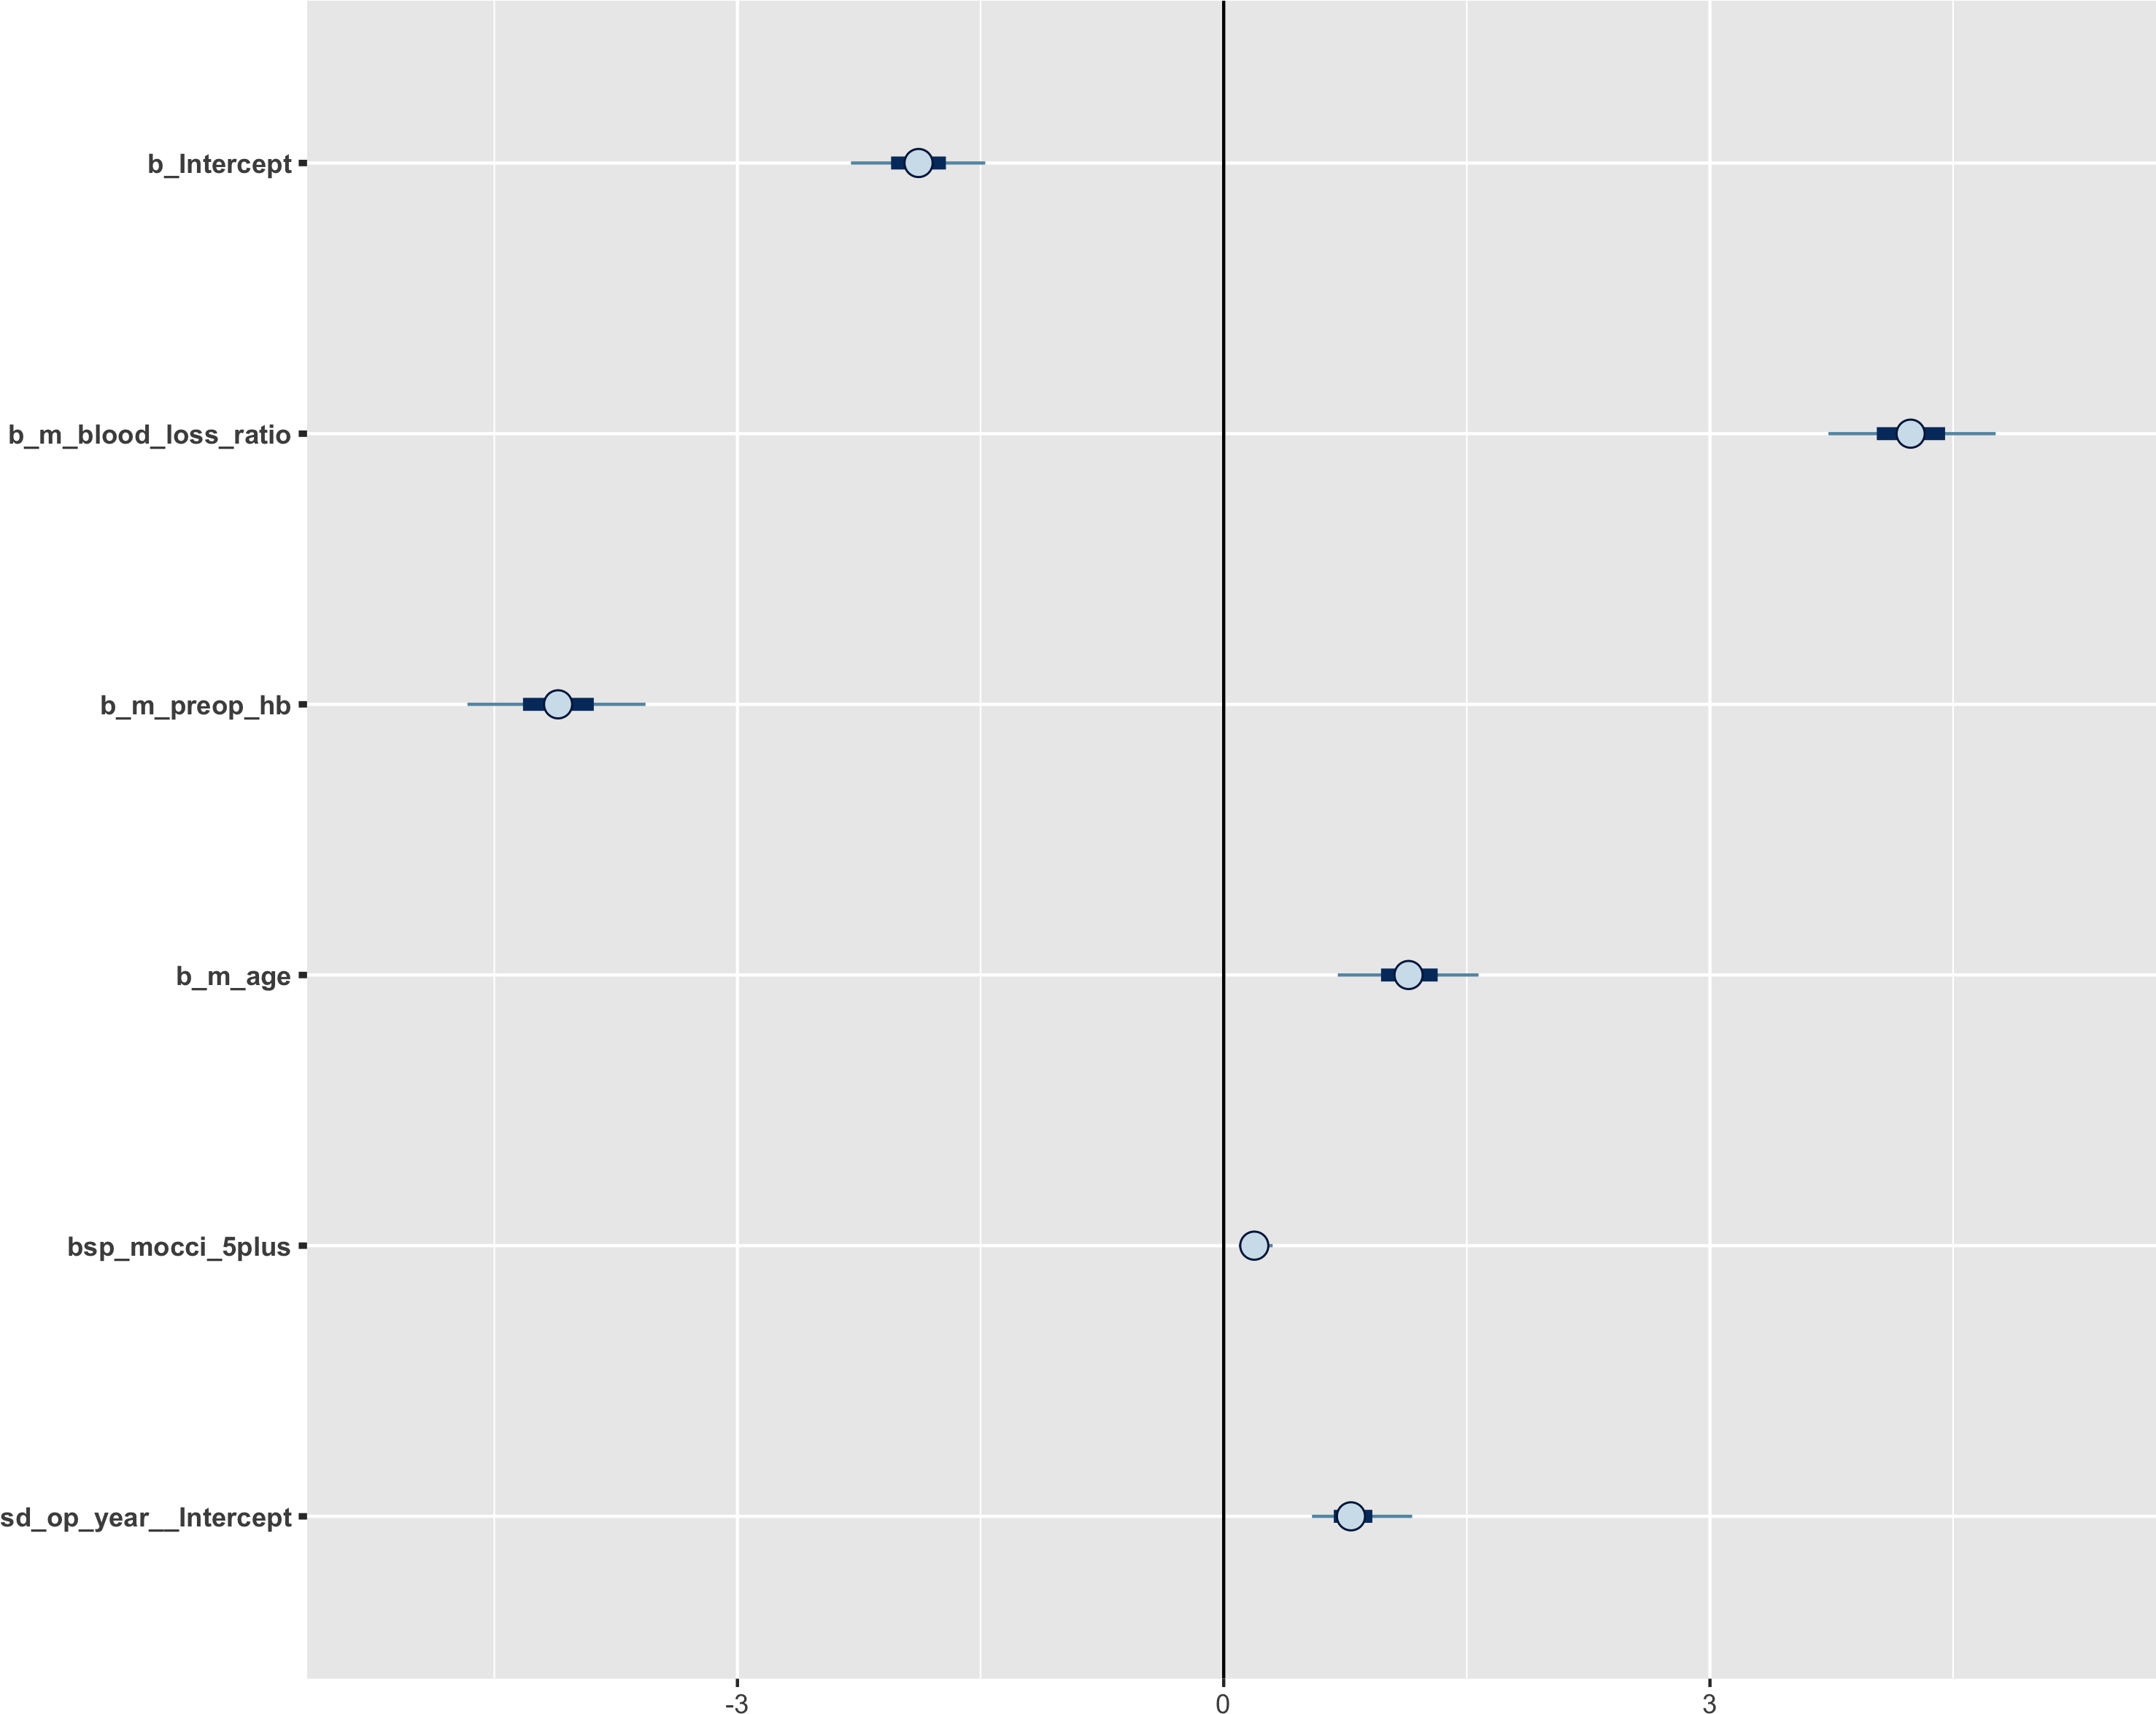
\includegraphics[width=1\linewidth]{notebook_files/figure-latex/model1reduced_diagnostics-2} \end{center}

\hypertarget{posterior-predictive-check-plot-1}{%
\subparagraph{Posterior predictive check plot}\label{posterior-predictive-check-plot-1}}

\begin{verbatim}
#> Using 10 posterior samples for ppc type 'bars' by default.
\end{verbatim}

\begin{center}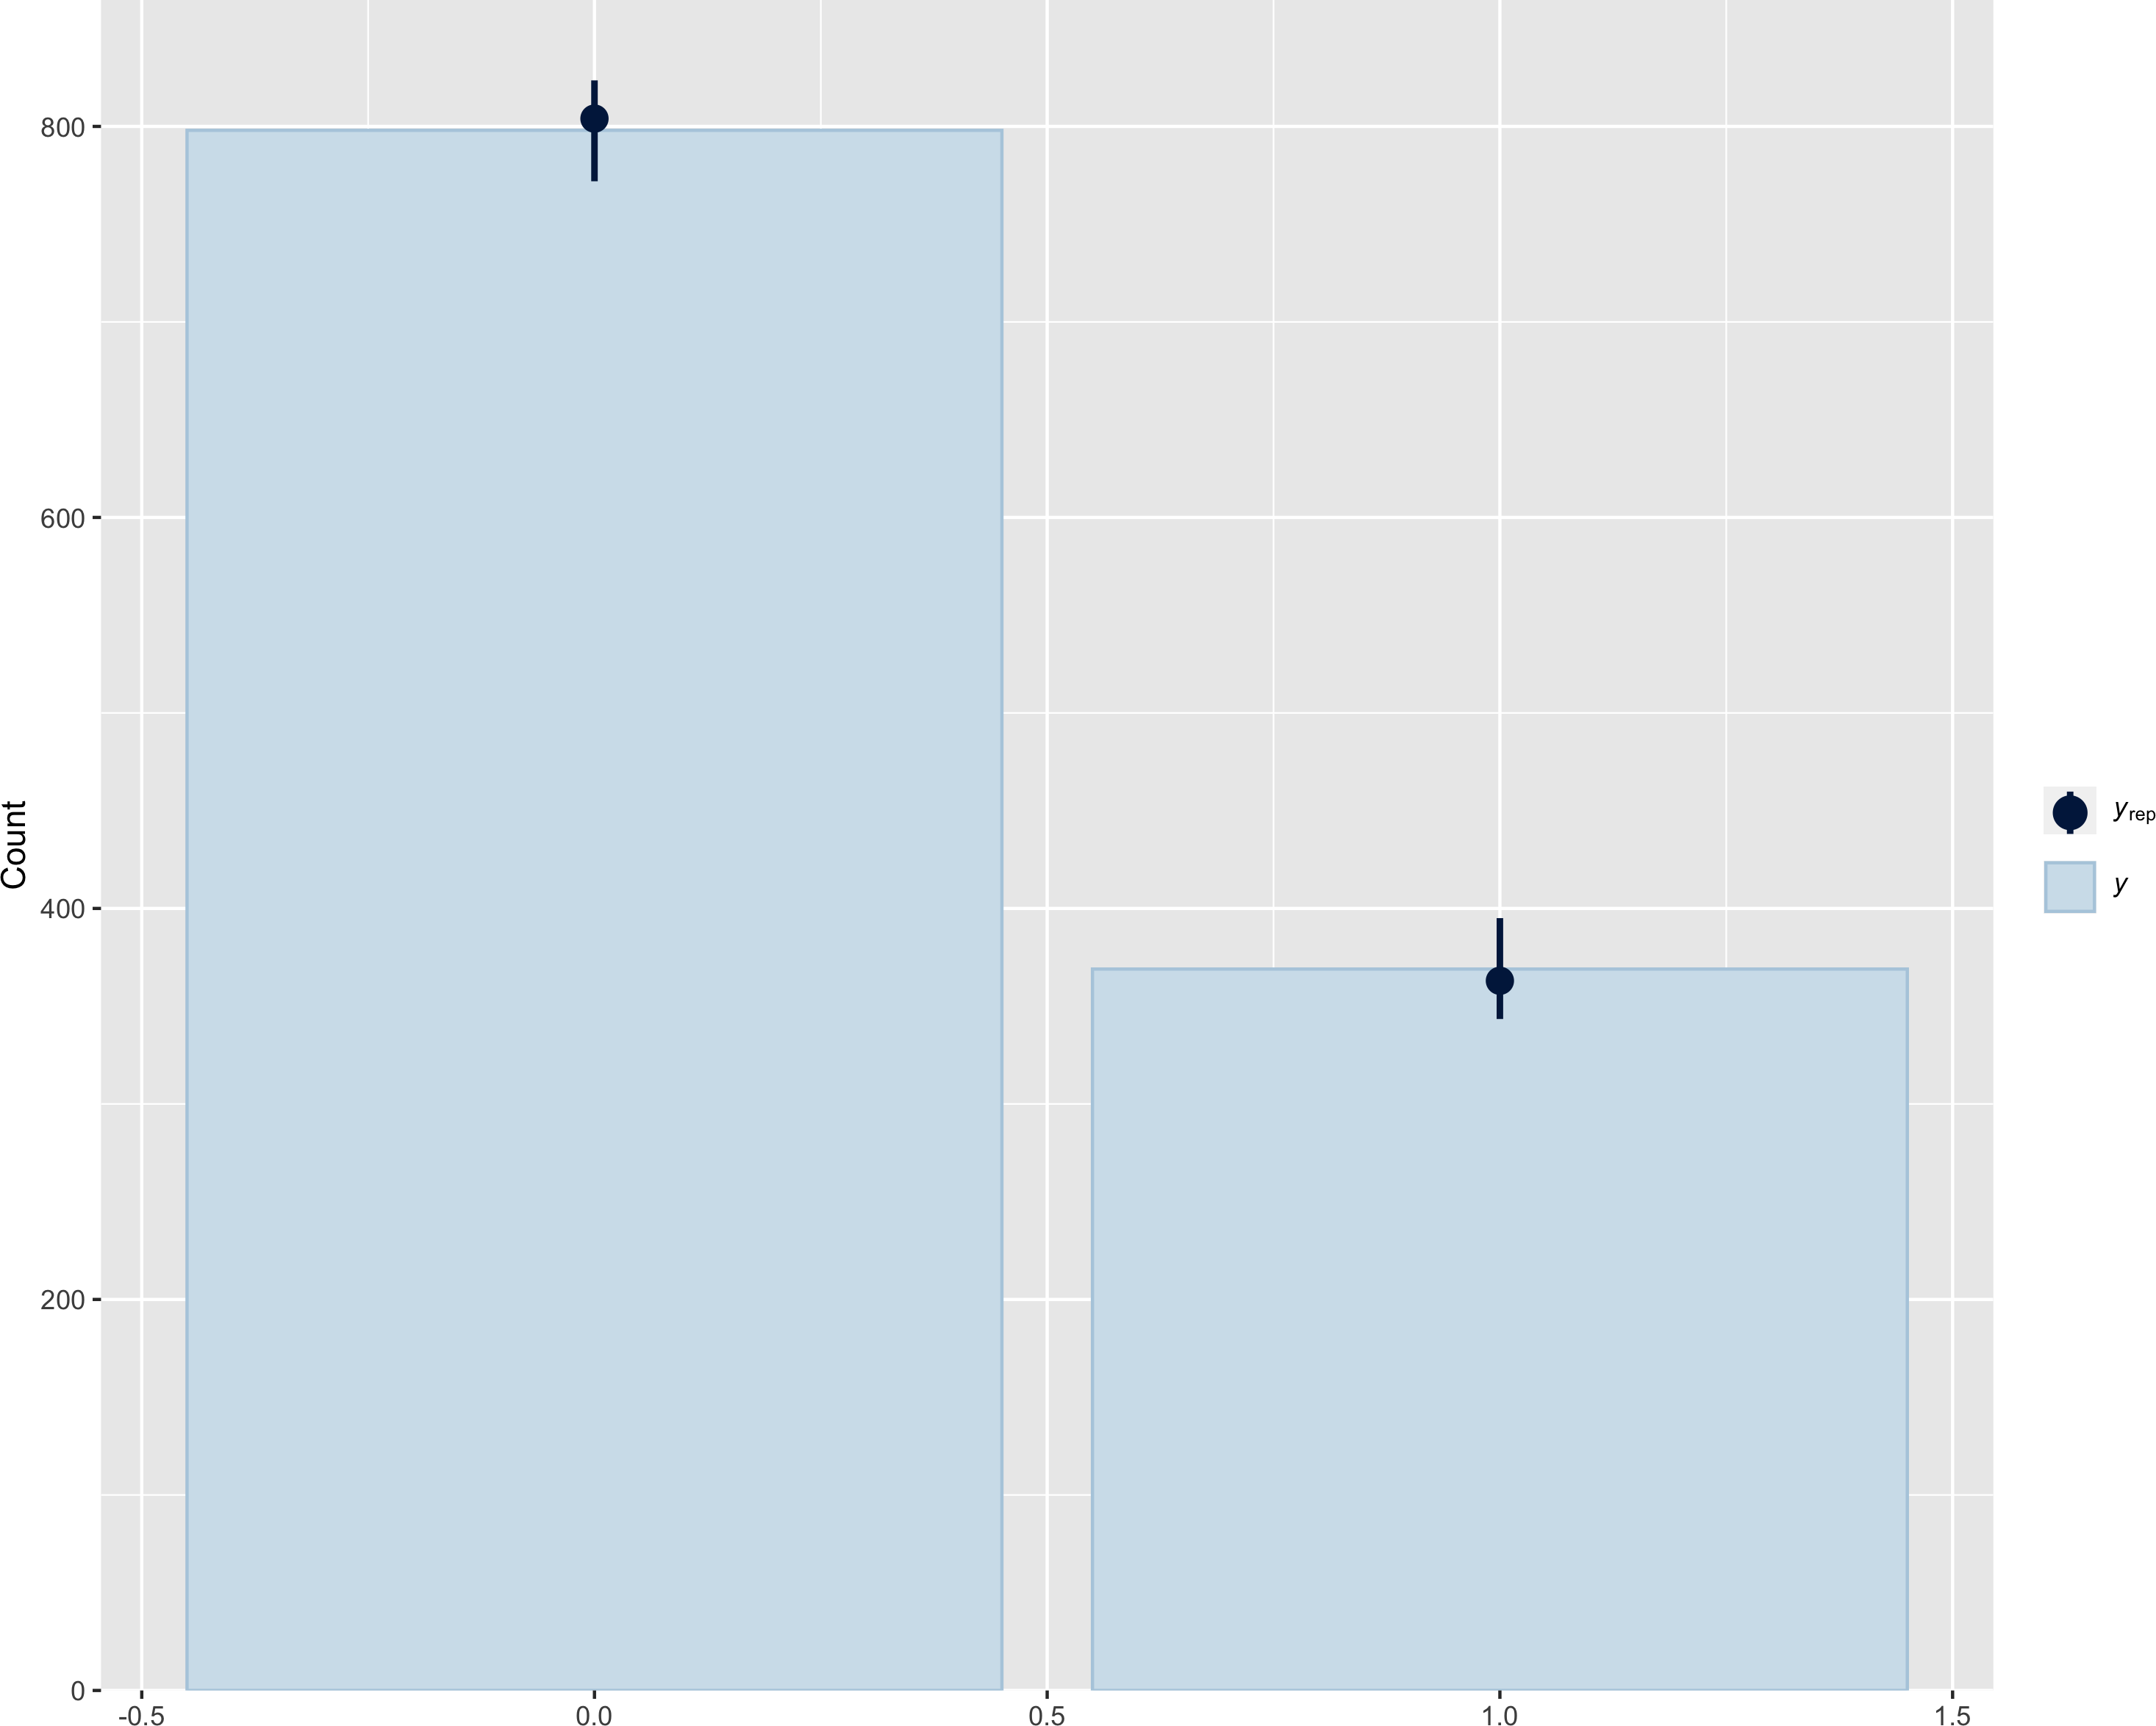
\includegraphics[width=1\linewidth]{notebook_files/figure-latex/model1reduced_ppcheck-1} \end{center}

\hypertarget{summary-1}{%
\subparagraph{Summary}\label{summary-1}}

\begin{verbatim}
#> # Description of Posterior Distributions
#> 
#> Parameter          | Median |           95% CI | p_MAP |    pd |       100% ROPE | % in ROPE
#> --------------------------------------------------------------------------------------------
#> Intercept          | -1.882 | [-2.380, -1.392] | 0.000 | 1.000 | [-0.055, 0.055] |     0.000
#> m_blood_loss_ratio |  4.238 | [ 3.631,  4.851] | 0.000 | 1.000 | [-0.055, 0.055] |     0.000
#> m_preop_hb         | -4.106 | [-4.753, -3.466] | 0.000 | 1.000 | [-0.055, 0.055] |     0.000
#> m_age              |  1.141 | [ 0.615,  1.642] | 0.000 | 1.000 | [-0.055, 0.055] |     0.000
#> mocci_5plus        |  0.189 | [ 0.062,  0.312] | 0.006 | 1.000 | [-0.055, 0.055] |     1.250
\end{verbatim}

\hypertarget{region-of-practical-equivalence-1}{%
\subparagraph{Region of practical equivalence}\label{region-of-practical-equivalence-1}}

Using a ROPE range of -0.055 to 0.055 (\(0.1 \cdot \frac{\sqrt{3}}{\pi}\)) and a CI of 1.

\begin{center}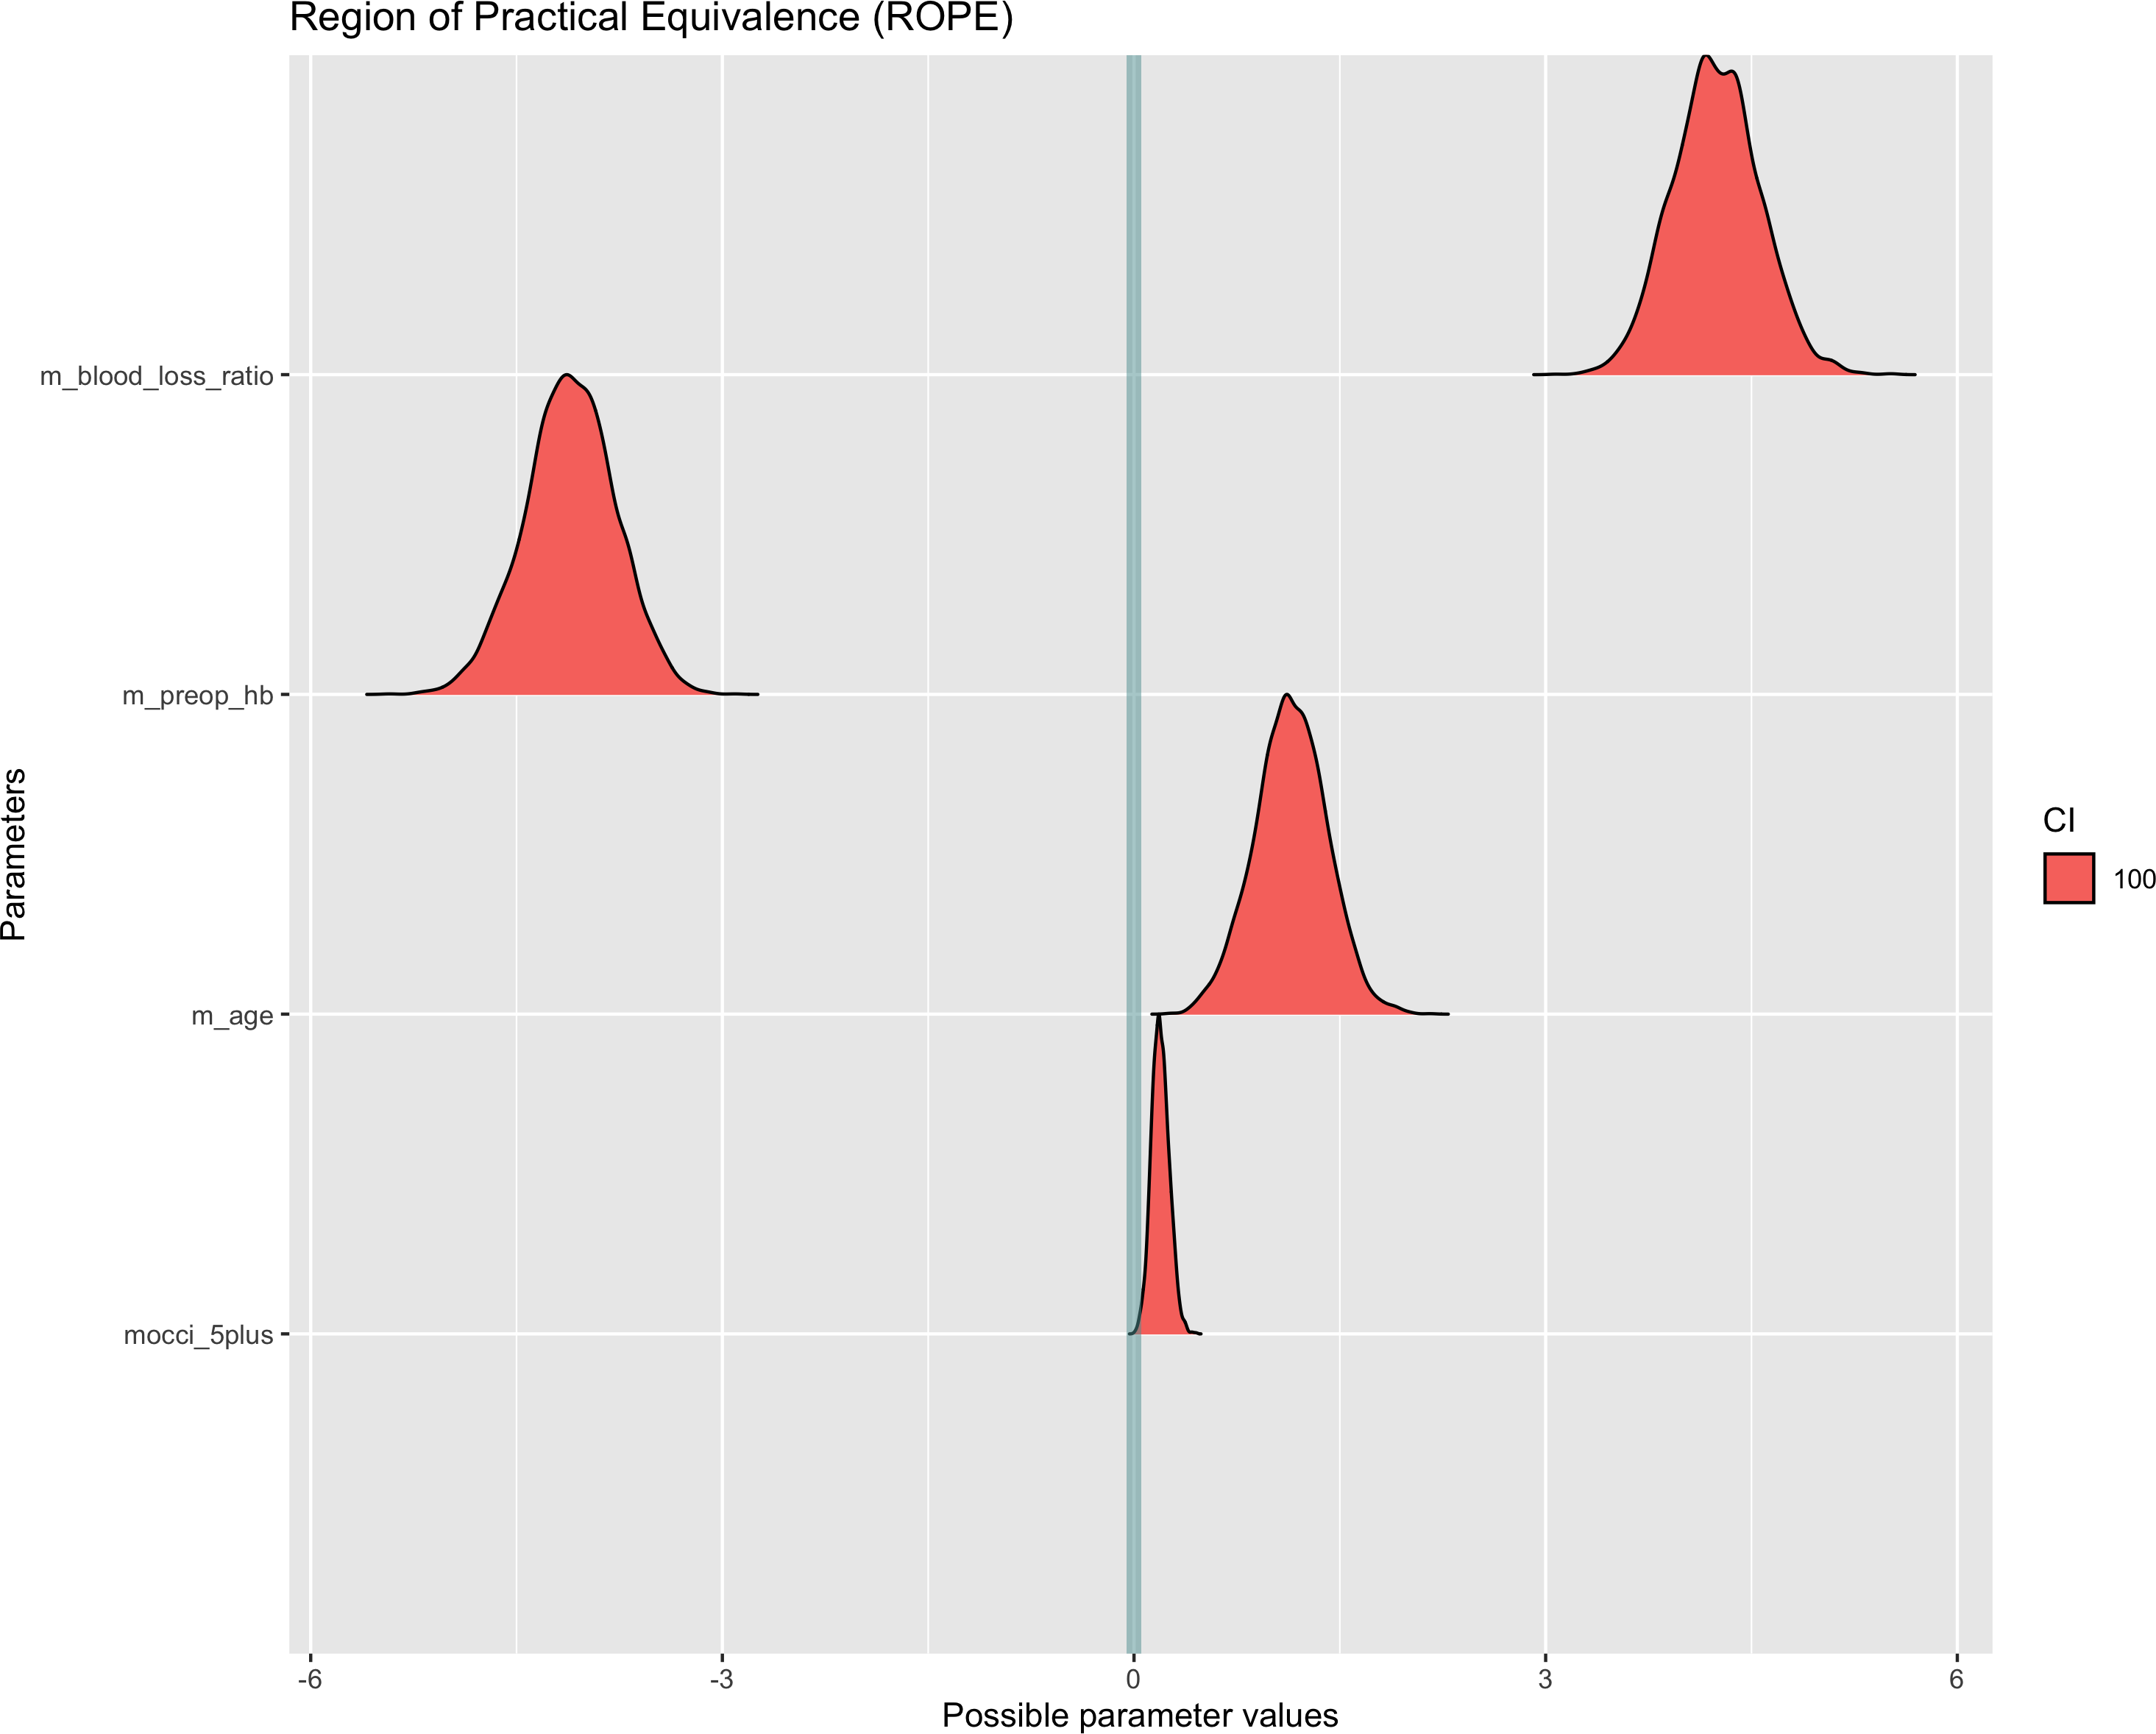
\includegraphics[width=1\linewidth]{notebook_files/figure-latex/model1reduced_rope-1} \end{center}

\hypertarget{roc-auc-1}{%
\subparagraph{ROC-AUC}\label{roc-auc-1}}

\begin{verbatim}
#> AUC: 0.873386039624811
\end{verbatim}

\begin{center}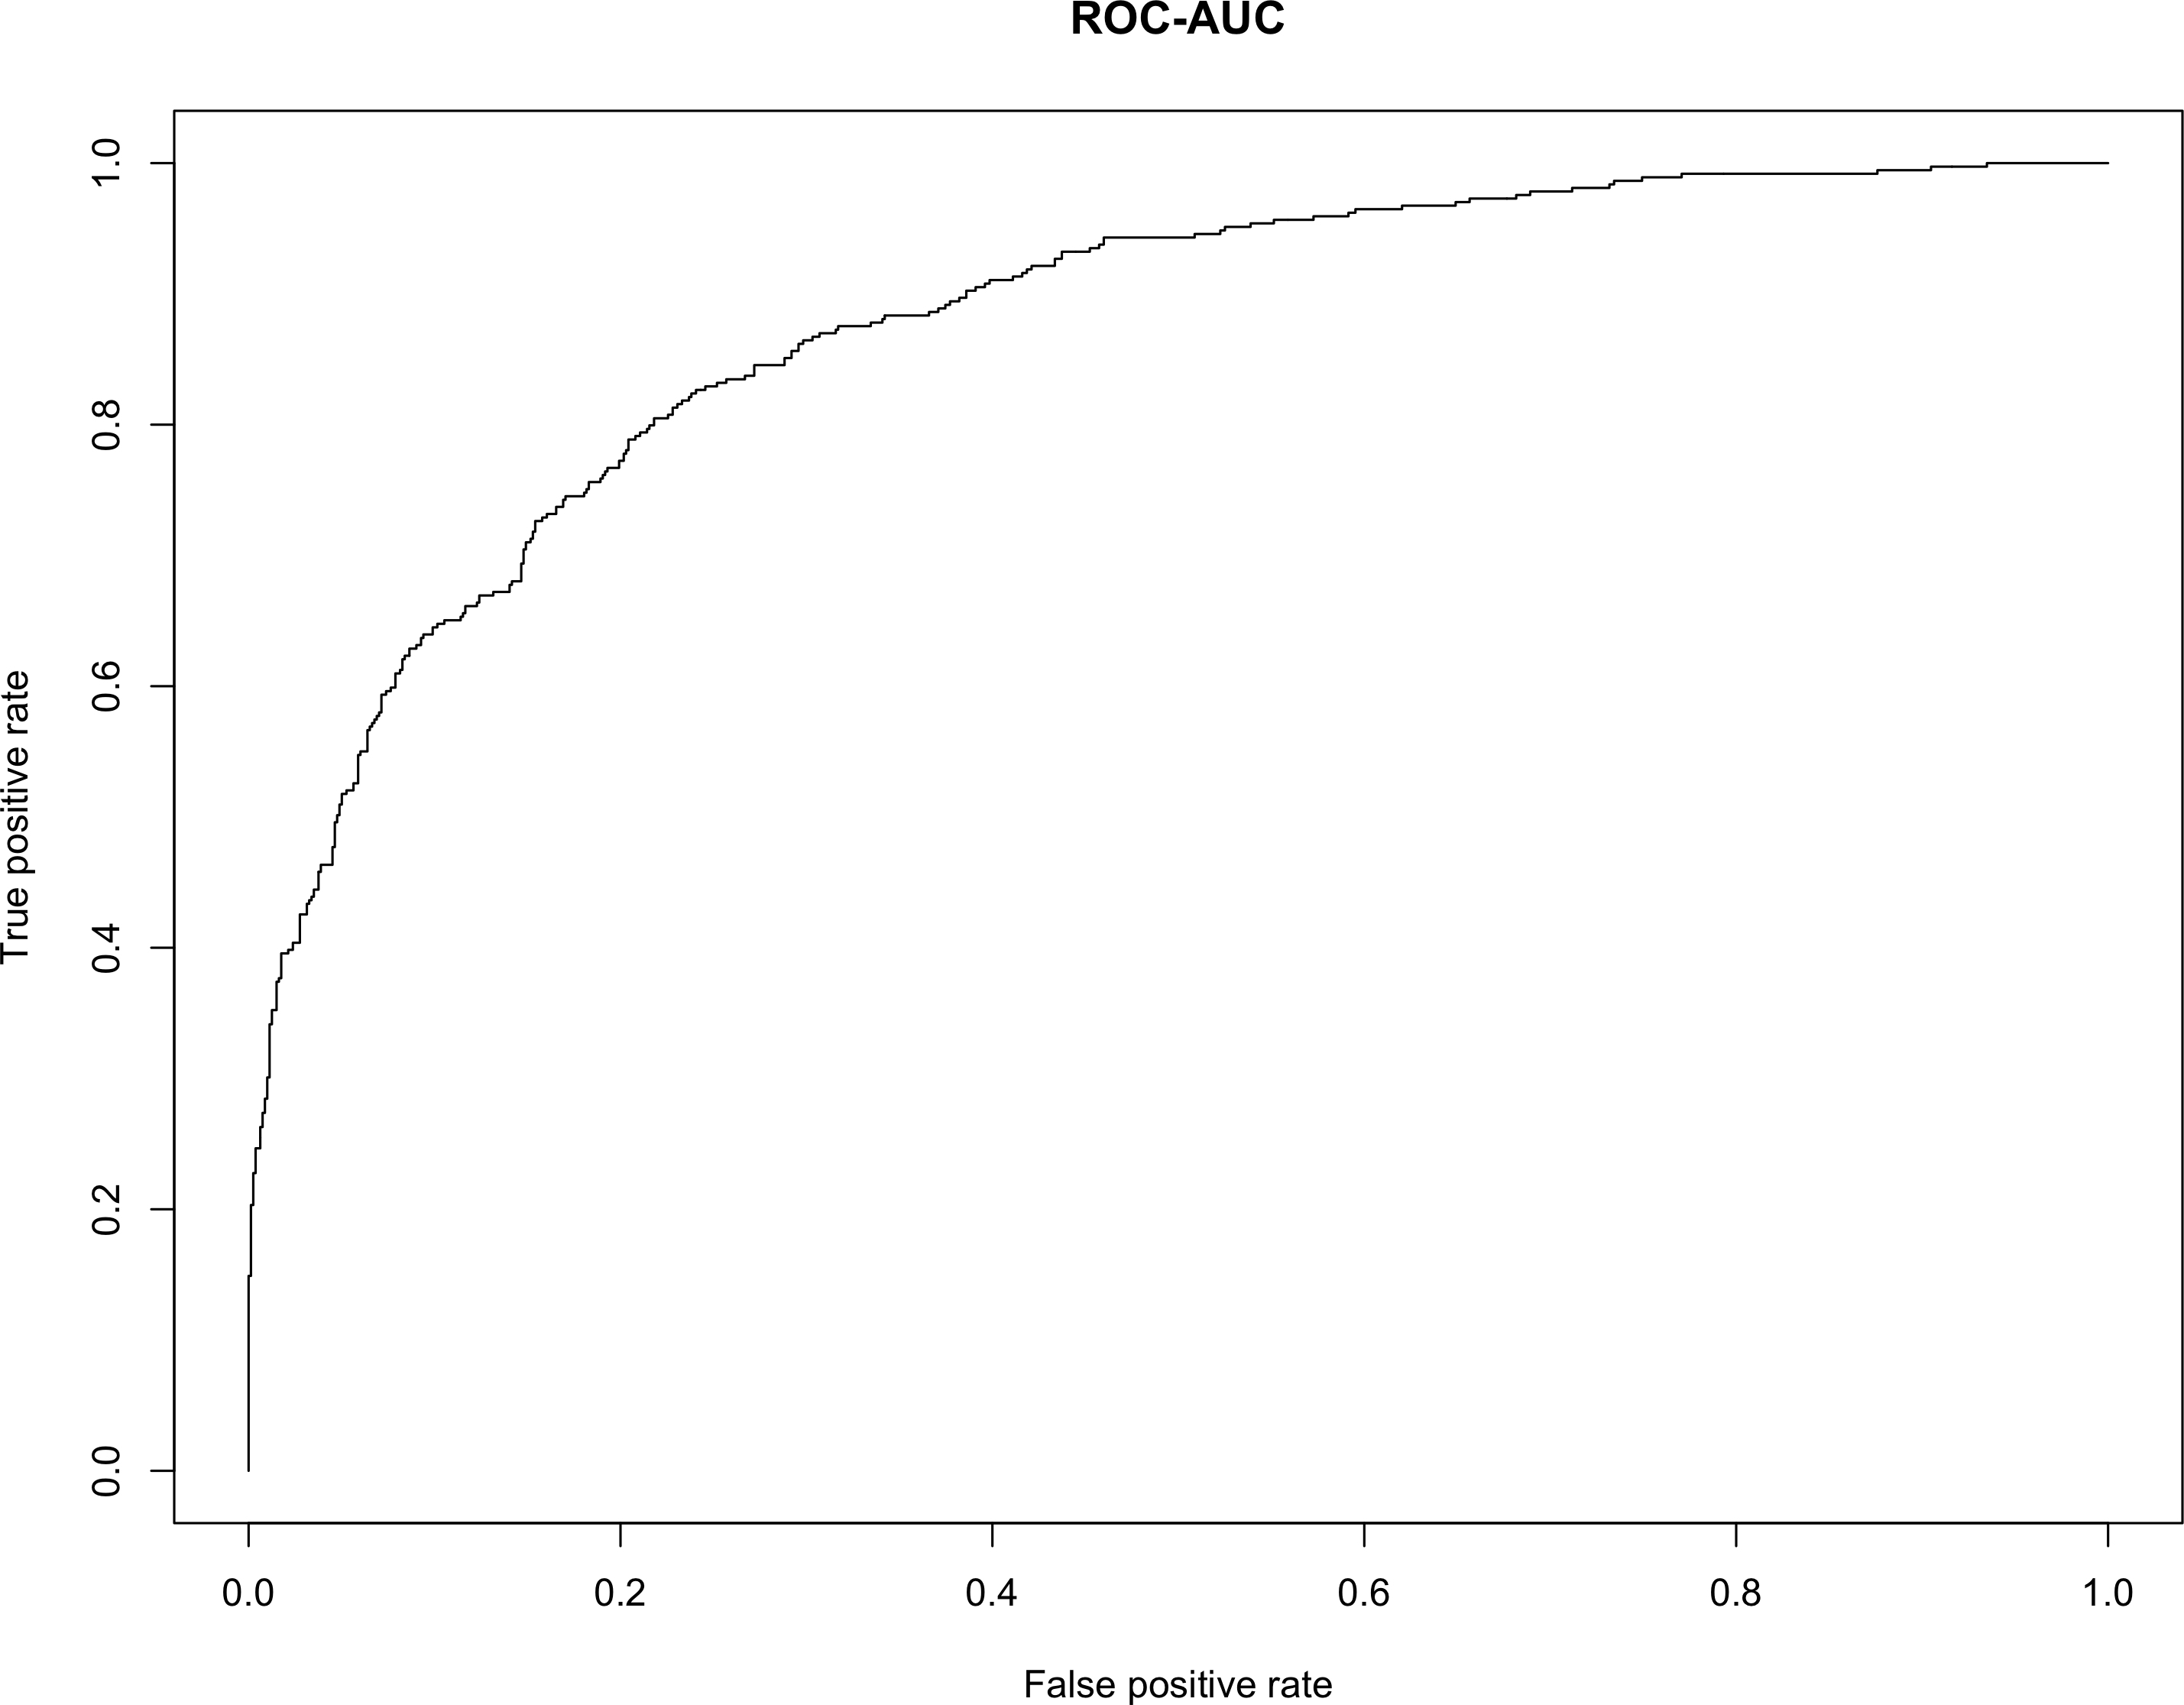
\includegraphics[width=1\linewidth]{notebook_files/figure-latex/model1reduced_rocauc-1} \end{center}

\hypertarget{conditional-probability-plot-1}{%
\subparagraph{Conditional probability plot}\label{conditional-probability-plot-1}}

\end{document}
